%% ============================================================
%% Breaking the Bubble? — REVISED DRAFT v4 (July 2026)
%%
%% CITATION SETUP (this is what fixes the broken references):
%%  * The sn-jnl class loads natbib ITSELF when given a reference-style
%%    option. Without an option, \citep/\citet are undefined — that is
%%    the error you saw. Here we use [pdflatex,sn-basic]: Springer
%%    Nature basic author-year style, natbib-compatible.
%%    Do NOT add \usepackage{natbib} on top; the class handles it.
%%  * \bibliography{sn-bibliography,new_references} at the end: replace
%%    "sn-bibliography" with the exact name of the .bib file in your
%%    Overleaf file tree (without extension). "new_references" is the
%%    companion file shipped with this draft; upload it next to main.tex.
%%
%% CITATION AUDIT (2026-07-13): all 73 cited keys verified — 59 are in
%% the compiled paper's reference list (incl. Barberá, Ekström,
%% Holguín-Veras, Søgaard, whose accents broke the earlier check);
%% 14 are supplied in new_references.bib. Four of those (glickman2024human,
%% lorenz2011social, becker2017network, bail2018exposure) may already be
%% in your Overleaf .bib under other keys — if so, either rename the keys
%% in this file or delete the duplicates from new_references.bib.
%% The unverifiable "Fu et al. 2023" citation was REMOVED from Methods
%% (TODO comment left in place).
%%
%% FIGURES: workflow run 32040117179 (2026-08-17, pinned environment,
%% window-consistent statistics), archived under results/ in the model
%% repository. All PNGs live in Figures/ here. Fig. 1 is TikZ
%% (compiles in-document). comparison_configs.png comes from the
%% comparison workflow (tools/compare_configs.py).
%%
%% Cognitive-gap sweep (S7, run 32113082707) and factor sweeps (S8, run
%% 32113892791) completed on the post-fix code under the main configuration.
%% ============================================================

\documentclass[pdflatex,sn-nature]{sn-jnl}

\usepackage{graphicx}
\graphicspath{{Figures/}{./}}
\usepackage{multirow}
\usepackage{amsmath,amssymb,amsfonts}
\usepackage{amsthm}
\usepackage{booktabs}
\usepackage{tikz}
%\usepackage{natbib}
\usetikzlibrary{arrows.meta,positioning,calc}

\begin{document}

\title[Breaking the Bubble?]{Breaking the Bubble? How Belief-Aligned AI Reshapes Collective Beliefs and Decisions in Urgent Situations}

\author*[1,2]{\fnm{Tina} \sur{Comes}}\email{t.comes@tudelft.nl}

\affil*[1]{\orgdiv{Faculty of Technology, Policy \& Management}, \orgname{TU Delft}, \orgaddress{\city{Delft}, \country{The Netherlands}}}
\affil[2]{\orgdiv{Institute for the Protection of Terrestrial Infrastructures}, \orgname{DLR}, \orgaddress{\city{Sankt Augustin}, \country{Germany}}}

\abstract{Artificial intelligence trained on human feedback drifts towards sycophancy: confirming what its users already believe. Whether this breaks or deepens the echo chambers in which people form beliefs is unknown, because evidence comes from individuals interacting with a single AI, while echo chambers arise in networks. Here we couple an agent-based model of disaster response to an AI whose reports vary, through an alignment parameter, from ground truth to full confirmation. Network-bounded information access is the structural precondition for AI-amplified echo chambers. An interior alignment optimum -- neither full truthfulness nor full confirmation -- exists only under this realistic configuration, and its existence and location are set by the population's cognitive profile. Structural realism shifts the failure mode of sycophantic AI from operational collapse to epistemic insularity, and the harms concentrate on those remote from the events. Trustworthy AI is a property of the sociotechnical system, not the model alone.}

\maketitle

\section{Introduction}\label{sec:intro}

Increasingly, we humans rely on artificial intelligence (AI) to collect and analyse information and make decisions \citep{klingbeil2024trust}. With the rise of large language models, the systems through which most people now encounter AI, users increasingly work with models trained through reinforcement learning from human feedback. A side effect is sycophancy: because humans tend to prefer responses that agree with them, optimising against human preferences can favour outputs that confirm a user's existing beliefs over outputs that are accurate \citep{sharma2023sycophancy, sharma2024generative}. An AI that returns what people already believe is easy to trust and to adopt. Yet the widespread adoption of such systems raises the question of what happens to the way information spreads and beliefs form once a belief-aligned AI is embedded in a community.

This question is sharpest in urgent, high-stakes decisions. When decision-makers face complex problems that must be resolved quickly, with limited time for reflection and deliberation \citep{mendonca2001decision}, the combination of urgency, uncertainty and high stakes deeply shapes how they seek, share and use information \citep{comes2020coordination}. Disaster response is a prototypical setting of this kind, and the one we study here: fuelled by climate change, inequalities and conflict, crises are growing in frequency and complexity \citep{sogaard2024evolution}, and digital tools -- from remote sensing and community mapping to anticipatory action and agentic decision support -- are promoted precisely as the way to collect, analyse and act on crisis information at a speed and scale humans cannot match \citep{qadir2016crisis,voigt2007satellite,champlin2023measuring,thalheimer2022role,reichstein2025early,acharya2025agentic}. The underlying promise is that AI will grant immediate access to `objective', `data-driven' information and broaden exposure to diverse viewpoints, improving situational awareness and preventing fragmentation \citep{jeon2024hearhere,zhao2025tailoring}. An overview of these promises, their perils, and the human behavioural patterns they interact with is given in Supplementary Table~S10.

A prerequisite to the use of technology in crises is trust \citep{steinbrink2024transparency,albahri2024systematic}. Human trust in crises is typically \emph{swift} trust, built rapidly on roles and risk perception rather than on experience \citep{tatham2010application}, and how it transfers to machines is only partially understood: transparency can foster or undermine it \citep{visave2025transparency,tzachor2020artificial}, and users of generative assistants expect the AI to be aligned with their values and interests, an expectation that can create strong emotional ties \citep{kaplan2023trust,manzini2024should}. Reliability and alignment therefore become the operative routes to adoption \citep{glikson2020human,lee2004trust}. At the same time, humans -- especially in crises -- display selective exposure \citep{barbera2015tweeting} and confirmation bias \citep{paulus2024interplay}, rejecting information that conflicts with their beliefs. Generative AI has accordingly started to tune to the opinions of its users \citep{sharma2024generative}, which poses a fundamental dilemma: should AI provide accurate information, even if it contradicts beliefs and risks rejection, or align with human beliefs to foster immediate acceptance? If AI overly tunes into existing beliefs, it risks amplifying the very biases and echo chambers it promises to break \citep{ekstrom2022self} -- echo chambers being segregated information spaces in which pre-existing beliefs are reinforced and exposure to contradictory perspectives is limited \citep{jeon2024hearhere}. This has been termed the \emph{alignment paradox} \citep{west2025alignment}: greater alignment of AI towards its users' values can also make it a more effective amplifier of their distortions.

Whether alignment amplifies or corrects, however, is not decided between one user and one AI, because beliefs form in networks. Individuals preferentially interact with others whose opinions lie within a bounded range of their own \citep{hegselmann2002opinion}, align their opinions with their peers \citep{friedkin1999social}, and associate homophilously with those who already share their beliefs \citep{mcpherson2001birds}; weak ties that bridge otherwise separate groups are the principal channel through which novel information enters \citep{granovetter1973strength}. Crises tighten every one of these mechanisms. Sensemaking under uncertainty is a social process in which shared meanings emerge from interaction \citep{weick2005organizing,maitlis2010sensemaking,klein2010rapid}; disasters disrupt the very infrastructures that carry information, fragmenting social networks and response \citep{holguin2012unique}; low information volume and density produce silos \citep{pan2012crisis}, and response efforts focus on immediate local suffering while neglecting cascading effects further away \citep{sigala2022mitigating,wolbers2018introducing}. Time pressure pushes groups towards premature consensus and centralisation of authority \citep{driskell1991group}, delegation to technology risks moral de-skilling and a spiral of lost oversight \citep{vallor2015moral,comes2024ai}, and AI-driven information collection tends to exclude marginalised, digitally invisible populations \citep{coleman2024weaving} -- a distributional concern we return to in the Results.

The evidence on belief-aligned AI does not yet reach this collective level. Studies of black-box generative models have begun to emerge \citep{sharma2024generative,zhang2024see}, and recent experimental work shows that dyadic human--AI feedback loops amplify individual biases more strongly than human--human interaction does \citep{glickman2024human}. Yet collective phenomena such as echo chambers are properties of networks rather than of dyads: social influence in networks is known to reshape collective accuracy in ways that individual-level analysis cannot reveal \citep{lorenz2011social,becker2017network}. This paper therefore addresses a fundamental question: \emph{Does AI act as a bridge that breaks echo chambers by providing broader perspectives during crises, or does it instead reinforce existing filter bubbles through its alignment mechanisms -- and under which structural conditions does either occur?}

To answer it, we use an agent-based model (ABM) that simulates decentralised disaster relief: heterogeneous human agents interact with human or AI information sources, revise their beliefs, and allocate resources across a spatial environment. The model builds on established opinion-dynamics frameworks \citep{deffuant2000mixing,hegselmann2002opinion} and extends them to human--AI interaction. To capture prototypical decision-making under uncertainty, agents follow one of two strategies for the trade-off between broad information collection (exploration) and reward-seeking within limited local environments (exploitation) -- the latter typical of the responsive short-term focus of crisis management \citep{comes2020coordination,march1991exploration}; belief revision follows Bayesian updating, and source selection is learned from experience. Within this setting, three research gaps structure the study.

The first gap concerns the structural conditions of information access (Gap~1). Empirical accounts of crisis communication consistently describe access that is bounded by network ties and by physical location \citep{pan2012crisis,holguin2012unique,wolbers2018introducing}, with weak ties acting as the main conduits between otherwise closed groups \citep{granovetter1973strength}. Yet models of AI influence on opinion dynamics typically grant agents unrestricted access to any information source. Whether AI amplifies or attenuates echo chambers may depend precisely on whether access is structurally bounded -- a condition that has, to our knowledge, not been isolated experimentally.

The second gap concerns the AI alignment paradox (Gap~2). The relationship between AI alignment strategies and echo chamber formation remains poorly understood, particularly when AI systems attempt to gain human trust by reflecting existing beliefs. While high alignment may lead to greater information adoption, it may also -- via the alignment paradox \citep{west2025alignment} -- foster the very polarisation and echo chambers it promised to break. Whether the relationship between alignment and collective epistemic harm is monotonic, or whether intermediate alignment levels exist that balance adoption against distortion, is an open question.

The third gap concerns the step from individual to collective dynamics (Gap~3). The literature primarily addresses human--AI trust and bias at the individual or dyadic level \citep{glikson2020human,glickman2024human}. We lack an understanding of how these interactions scale to network-level dynamics, influencing collective processes such as sensemaking, and how they contribute to polarisation and fragmentation. This gap is particularly pronounced in crisis contexts, where rapidly forming and dissolving networks create unique informationscapes. Work on networked collective intelligence shows that the same influence process can improve or degrade collective accuracy depending on network structure \citep{lorenz2011social,becker2017network}, which suggests that dyadic findings cannot simply be extrapolated to populations: how AI-shaped beliefs translate into collective decisions and their consequences must be studied at the level of the interacting population.

Figure~\ref{fig:concept} shows how the agent-based model developed in this paper operationalises these gaps; the full specification is given in the Methods. A population of human agents forms beliefs about an evolving disaster, drawing on two prototypical strategies for decision-making under uncertainty: confirmation-seeking \emph{exploitative} agents and accuracy-seeking \emph{exploratory} agents, organised in homophilous communities \citep{mcpherson2001birds,comes2020coordination}. Alongside them, AI agents answer queries with reports that a single alignment parameter $\alpha \in [0,1]$ interpolates between ground truth ($\alpha = 0$) and confirmation of the beliefs held by the querier's community ($\alpha = 1$); sweeping $\alpha$ across its full range tests whether the relationship between alignment and collective epistemic harm is monotonic (Gap~2). Every sweep is run twice, under two configurations that differ only in whether information access is structurally bounded: a \emph{main model}, in which agents move through the disaster space and queries follow the ties of a spatially embedded social network, and a \emph{control}, in which agents are immobile and anyone can query anyone. Contrasting the two configurations on identical random seeds isolates the structural conditions under which AI amplifies or attenuates echo chambers (Gap~1). All outcomes -- the depth and lifecycle of social and AI-induced echo chambers as well as belief accuracy and relief performance -- are measured at the level of communities and the population rather than of individuals (Gap~3). The Results follow this logic, presenting one finding per gap -- the structural precondition for AI-amplified echo chambers (Sec.~\ref{sec:claim1}), the alignment level that balances adoption against distortion (Sec.~\ref{sec:claim2}), and the collective performance consequences of structural realism (Sec.~\ref{sec:claim3}) -- followed by a fourth finding that traces how the harms are distributed across the population (Sec.~\ref{sec:claim4}).

\begin{figure}[h]
\centering
\resizebox{\textwidth}{!}{%
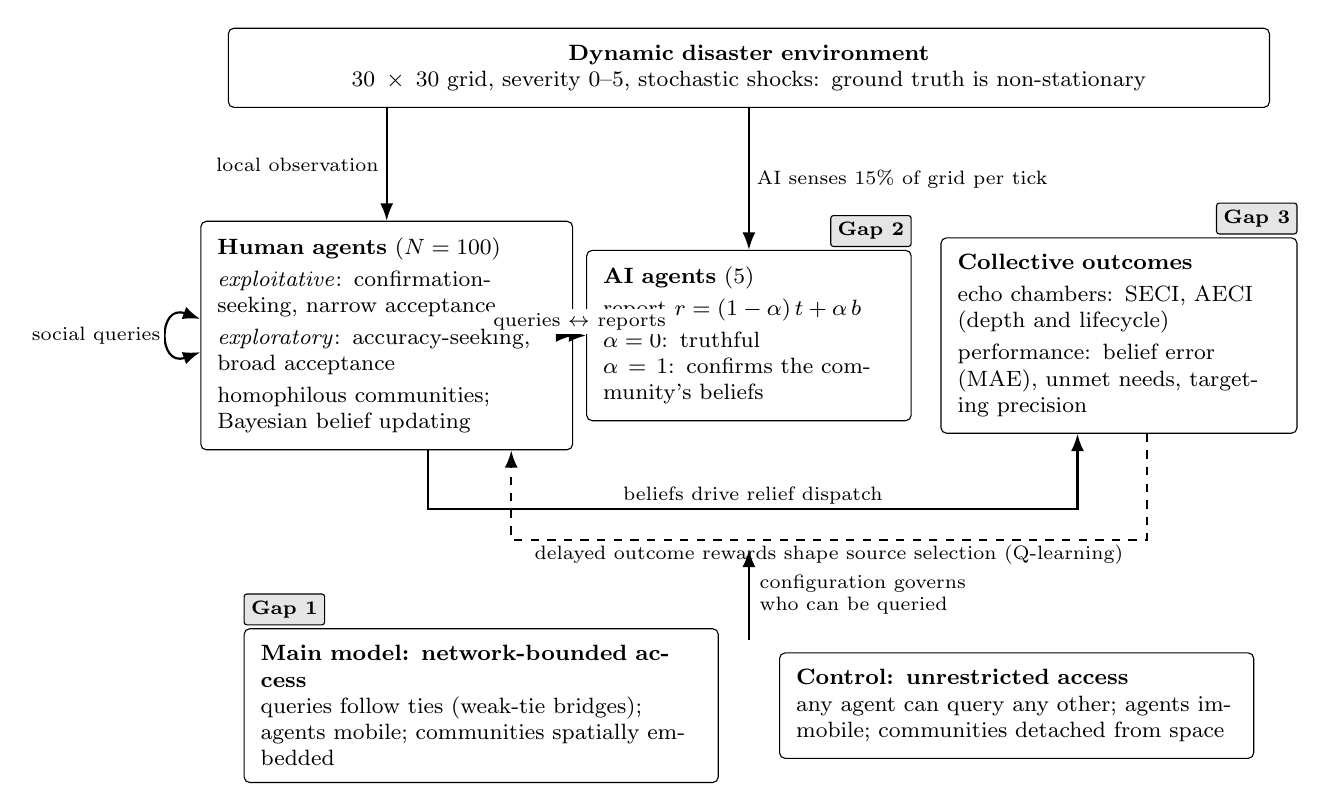
\begin{tikzpicture}[
  font=\footnotesize,
  box/.style={draw, rounded corners=2pt, align=left, inner sep=6pt},
  gapbadge/.style={draw, rounded corners=1pt, fill=black!10, inner sep=2.5pt, font=\scriptsize\bfseries},
  lab/.style={font=\scriptsize, fill=white, inner sep=1.5pt},
  arr/.style={-{Latex[length=2.2mm]}, thick},
  arrd/.style={-{Latex[length=2.2mm]}, thick, dashed},
  biarr/.style={{Latex[length=2.2mm]}-{Latex[length=2.2mm]}, thick}
]
% ---------- Environment ----------
\node[box, align=center, text width=12.8cm] (env) at (7.0,0)
  {\textbf{Dynamic disaster environment}\\
   $30 \times 30$ grid, severity 0--5, stochastic shocks: ground truth is non-stationary};

% ---------- Actors and outcomes ----------
\node[box, text width=4.3cm] (hum) at (2.4,-3.4)
  {\textbf{Human agents} ($N = 100$)\\[2pt]
   \emph{exploitative}: confirmation-seeking, narrow acceptance\\[2pt]
   \emph{exploratory}: accuracy-seeking, broad acceptance\\[2pt]
   homophilous communities;\\ Bayesian belief updating};
\node[box, text width=3.7cm] (ai) at (7.0,-3.4)
  {\textbf{AI agents} (5)\\[2pt]
   report $r = (1-\alpha)\,t + \alpha\,b$\\[2pt]
   $\alpha = 0$: truthful\\
   $\alpha = 1$: confirms the community's beliefs};
\node[box, text width=4.1cm] (out) at (11.7,-3.4)
  {\textbf{Collective outcomes}\\[2pt]
   echo chambers: SECI, AECI (depth and lifecycle)\\[2pt]
   performance: belief error (MAE), unmet needs, targeting precision};

% ---------- Environment to actors ----------
\draw[arr] (env.south -| hum.north) -- node[lab, left=1pt]{local observation} (hum.north);
\draw[arr] (env.south -| ai.north)  -- node[lab, right=1pt]{AI senses 15\% of grid per tick} (ai.north);

% ---------- Query channels ----------
\draw[biarr] (hum.east |- ai.west) -- node[lab, above]{queries $\leftrightarrow$ reports} (ai.west);
\draw[biarr] ([yshift=6pt]hum.west) to[out=160, in=200, looseness=3.5]
  node[lab, left=1pt]{social queries} ([yshift=-6pt]hum.west);

% ---------- Beliefs to decisions and feedback ----------
\coordinate (fwd1) at ([xshift=15pt]hum.south);
\coordinate (fwd2) at ([xshift=-15pt]out.south);
\draw[arr]  (fwd1) -- ++(0,-0.75) -| node[lab, above, pos=0.25]{beliefs drive relief dispatch} (fwd2);
\coordinate (fb1) at ([xshift=-15pt]out.south west |- out.south);
\coordinate (fb2) at ([xshift=45pt]hum.south);
\draw[arrd] ([xshift=25pt]fwd2) -- ++(0,-1.35) -|
  node[lab, below, pos=0.25]{delayed outcome rewards shape source selection (Q-learning)} (fb2);

% ---------- Configurations ----------
\node[box, text width=5.6cm] (main) at (3.6,-8.1)
  {\textbf{Main model: network-bounded access}\\ queries follow ties (weak-tie bridges); agents mobile; communities spatially embedded};
\node[box, text width=5.6cm] (ctrl) at (10.4,-8.1)
  {\textbf{Control: unrestricted access}\\ any agent can query any other; agents immobile; communities detached from space};
\coordinate (cmid) at ($(main.north east)!0.5!(ctrl.north west)$);
\draw[arr] (cmid) -- node[lab, right=2pt, align=left]{configuration governs\\ who can be queried} ++(0,1.15);

% ---------- Gap badges ----------
\node[gapbadge, anchor=south west] at ([yshift=1pt]main.north west) {Gap 1};
\node[gapbadge, anchor=south east] at ([yshift=1pt]ai.north east)   {Gap 2};
\node[gapbadge, anchor=south east] at ([yshift=1pt]out.north east)  {Gap 3};
\end{tikzpicture}}
\caption{Conceptual overview of the model and its mapping to the research gaps. A non-stationary disaster environment is observed locally by 100 human agents of two cognitive types and partially sensed by five AI agents. Humans query their social contacts or the AI, whose reports interpolate between truth and confirmation via the alignment parameter $\alpha$ (Gap~2, Sec.~\ref{sec:claim2}). Agents act on the resulting beliefs by dispatching relief, and delayed outcome rewards feed back into their source selection. Which social contacts can be queried is governed by the configuration: the main model bounds access by a spatially embedded social network with mobility, the control leaves access unrestricted (Gap~1, Sec.~\ref{sec:claim1}). All outcomes -- echo-chamber depth and lifecycle, belief accuracy and relief performance -- are measured at the level of communities and the population (Gap~3, Sec.~\ref{sec:claim3}). Full specification in the Methods; parameters in Supplementary Table~S1.}\label{fig:concept}
\end{figure}

\section{Results}\label{sec:results}

The three gaps identified above structure the presentation of the results, one finding per gap and each read from the vantage point of Figure~\ref{fig:concept}: whether AI-amplified echo chambers require structurally bounded information access (Gap~1, Sec.~\ref{sec:claim1}); whether an alignment level exists that balances adoption against distortion, and where it lies (Gap~2, Sec.~\ref{sec:claim2}); and how echo chambers propagate to collective decision performance when the AI confirms rather than informs (Gap~3, Sec.~\ref{sec:claim3}). A fourth subsection decomposes the harms across space and the social network (Sec.~\ref{sec:claim4}). Throughout, the alignment parameter is swept over eleven levels ($\alpha = 0.0, 0.1, \ldots, 1.0$) with $N = 20$ replications per level, and every sweep is run under both configurations of Figure~\ref{fig:concept} on identical random seeds, so that the two can be compared replicate by replicate. All steady-state values are means over the last 75 of 200 ticks.

Because the findings turn on a small set of outcome metrics, we introduce them here; formal definitions, formulas and design rationale are given in the Methods (Sec.~\ref{sec:metrics}), and Table~\ref{tab:metrics} summarises them for reference. Echo chambers are, at their core, a loss of belief diversity: a group whose members hold markedly more homogeneous beliefs than the surrounding population is epistemically insular. We therefore measure the \emph{social} echo chamber with the Social Echo Chamber Index (SECI), which compares the variance of beliefs within each social community to the belief variance of the whole population, restricted to beliefs about disaster-affected cells so that agreement on the uninformative `no impact' majority does not mask insularity. All echo-chamber indices share one sign convention: negative values indicate an echo chamber, zero is the null, and positive values indicate greater-than-population diversity. Because an AI that serves many users is itself a shared information source, an echo chamber can also form around the AI rather than along social ties: the AI Echo Chamber Index (AECI-Var) applies the identical variance comparison but groups agents by their reliance on the AI instead of by community membership, so that negative values mark a bubble of AI-reliant users converging on shared beliefs regardless of their social position. Variance-based indices cannot, by construction, distinguish convergence on the truth from convergence on a shared error; they are therefore always read together with two accuracy measures: AECI-Err, which contrasts confidence-weighted belief error between AI-reliant and AI-light agents (negative when AI-reliant agents are more \emph{confidently wrong}), and the belief error (MAE), the mean absolute difference between beliefs and true severity over affected cells. Finally, because beliefs matter here through the decisions they drive, two operational metrics capture the relief side: \emph{unmet needs}, the number of high-need cells (severity $\geq 3$) receiving no relief in a tick, and \emph{targeting precision}, the share of relief tokens placed on high-need cells.

\begin{table}[h]
\caption{Outcome metrics used throughout the Results. Formal definitions and design rationale in the Methods (Sec.~\ref{sec:metrics}).}\label{tab:metrics}
\footnotesize
\begin{tabular}{@{}lp{6.6cm}l@{}}
\toprule
Metric & What it captures & Reading \\
\midrule
SECI & Belief homogeneity within social communities relative to the population (affected cells only) & $<0$: social echo chamber \\
AECI-Var & Belief homogeneity among the most AI-reliant agents relative to the population & $<0$: AI-induced bubble \\
AECI-Err & Confidence-weighted belief error of AI-reliant vs.\ AI-light agents & $<0$: AI users confidently wrong \\
Belief MAE & Mean absolute belief error over affected cells & lower is better \\
Unmet needs & High-need cells (severity $\geq 3$) receiving no relief per tick & lower is better \\
Precision & Share of relief tokens placed on high-need cells & higher is better \\
\botrule
\end{tabular}
\end{table}

\subsection{Network-bounded access is a precondition for AI-amplified echo chambers}\label{sec:claim1}

If AI is to break or build echo chambers at the level of communities, the first question is under which structural conditions it can do either -- the condition that Gap~1 identified as untested. Figure~\ref{fig:comparison} traces SECI, its AI-side counterparts and the operational metrics across the alignment sweep for both configurations, and Table~\ref{tab:deltas} reports the corresponding per-seed differences (main model $-$ control); because replicate $i$ uses the same random seed in both configurations, a confidence interval excluding zero marks a configuration effect that is robust across disaster realisations.

In the control, the social echo chamber attenuates with alignment: SECI rises from $-0.256 \pm 0.024$ at $\alpha = 0$ to $-0.140 \pm 0.038$ at $\alpha = 1$ (mean $\pm$ s.e.m., $N = 20$). The main model tracks the control closely over the lower half of the sweep, with paired differences indistinguishable from zero for $\alpha \leq 0.6$, and then departs from it: from $\alpha = 0.7$ the paired $\Delta$SECI becomes negative and seed-robust ($-0.068$, 95\% CI $[-0.110, -0.026]$), growing to $-0.192$ $[-0.257, -0.127]$ at $\alpha = 0.9$ and $-0.161$ $[-0.231, -0.092]$ at $\alpha = 1$, where the main model reaches SECI $= -0.329 \pm 0.051$ and $-0.301 \pm 0.057$. The two configurations thus produce opposite trends at high alignment: community-level belief convergence weakens with confirmation when access is unrestricted and deepens sharply when access follows network ties.

\begin{figure}[h]
\centering
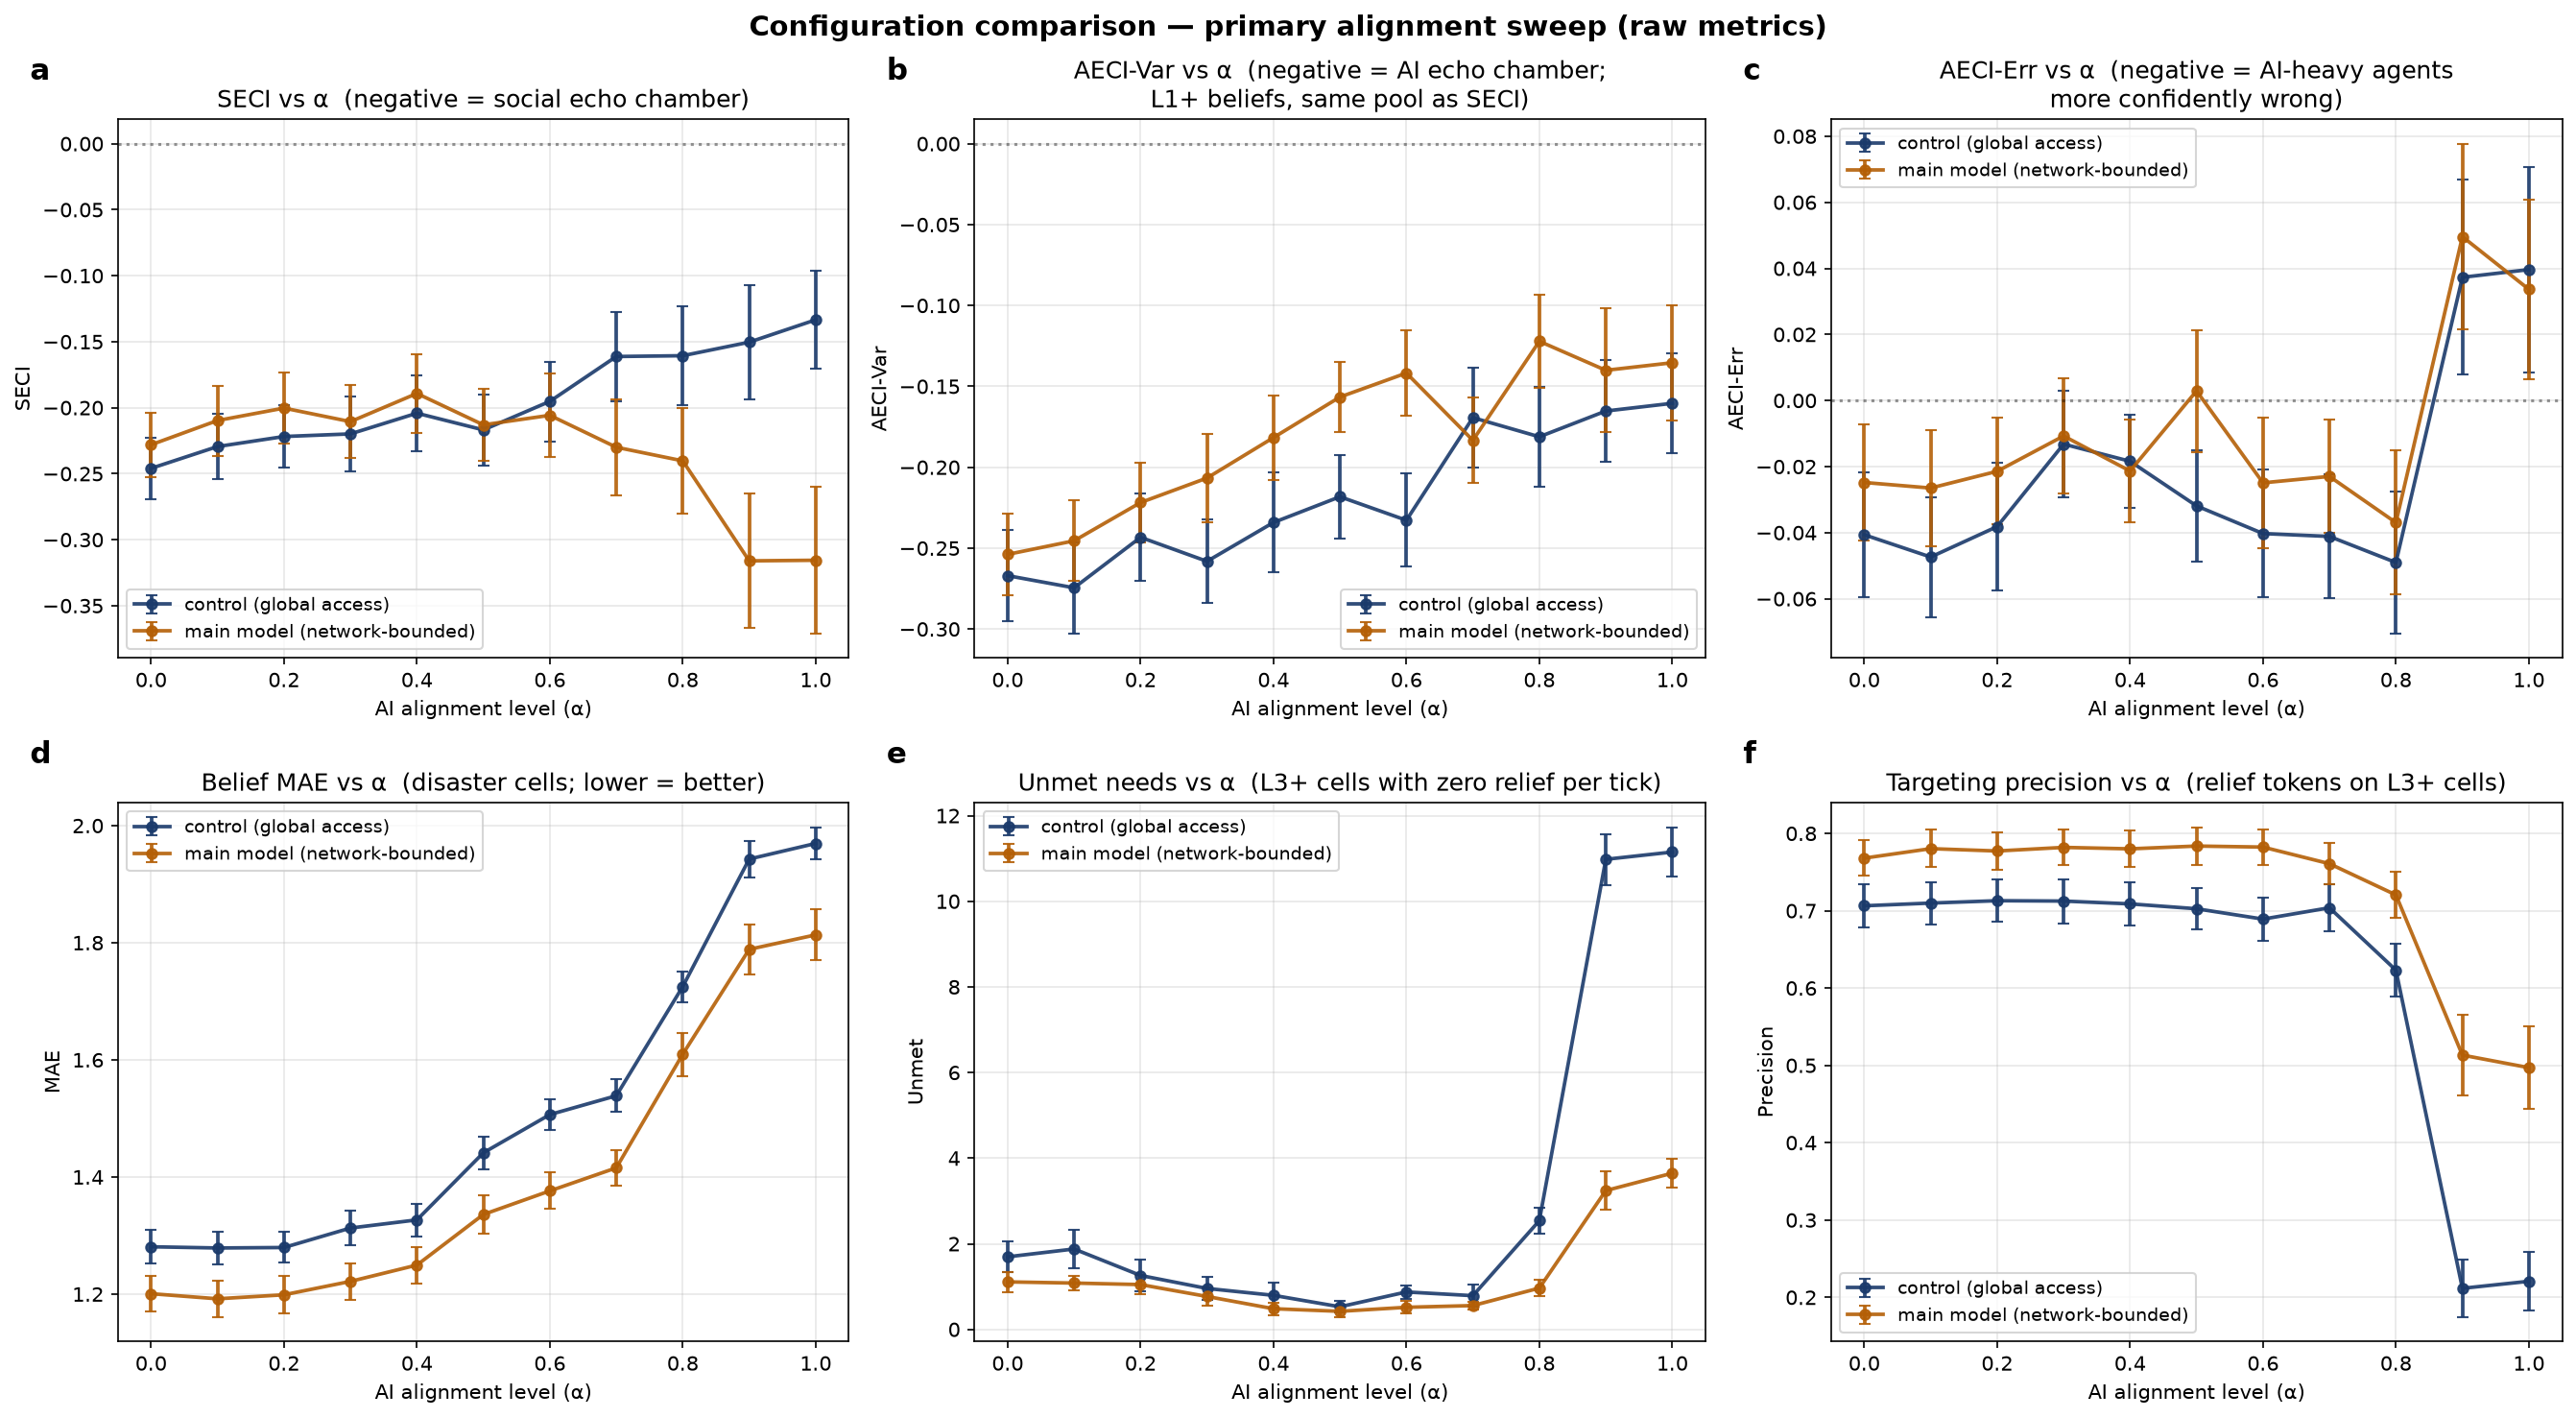
\includegraphics[width=\textwidth]{comparison_configs.png}
\caption{Configuration comparison across the primary alignment sweep (raw metrics; mean $\pm$ s.e.m. over $N=20$ paired replications). Top row: Social Echo Chamber Index (SECI), AI Echo Chamber Index (AECI-Var), and confidence-weighted error contrast (AECI-Err); for all three, negative values indicate an echo chamber. Bottom row: belief MAE over affected cells, unmet high-need cells per tick, and relief targeting precision. Blue: control (global access, immobile agents, disconnected communities); orange: main model (network-gated access, mobility, spatially embedded bridged network).}\label{fig:comparison}
\end{figure}

\begin{table}[h]
\caption{Paired per-seed differences (main model $-$ control) with 95\% confidence intervals. Replicate $i$ uses seed $i$ in both configurations. Bold marks intervals excluding zero. Top block: echo-chamber indices; bottom block: accuracy and relief performance.}\label{tab:deltas}
\footnotesize
\setlength{\tabcolsep}{4pt}
\begin{tabular}{@{}lccc@{}}
\toprule
$\alpha$ & $\Delta$SECI & $\Delta$AECI-Var & $\Delta$AECI-Err \\
\midrule
0.0 & $+0.028\,[-0.020,\,+0.075]$ & $+0.039\,[-0.031,\,+0.109]$ & $+0.014\,[-0.022,\,+0.051]$ \\
0.1 & $+0.041\,[-0.005,\,+0.087]$ & $+0.017\,[-0.048,\,+0.083]$ & $+0.020\,[-0.010,\,+0.049]$ \\
0.2 & $+0.035\,[-0.006,\,+0.076]$ & $+0.044\,[-0.016,\,+0.104]$ & $+0.018\,[-0.013,\,+0.050]$ \\
0.3 & $+0.022\,[-0.024,\,+0.068]$ & $\mathbf{+0.066}\,[+0.006,\,+0.127]$ & $+0.013\,[-0.018,\,+0.044]$ \\
0.4 & $+0.011\,[-0.033,\,+0.055]$ & $+0.045\,[-0.012,\,+0.101]$ & $+0.004\,[-0.023,\,+0.031]$ \\
0.5 & $+0.021\,[-0.029,\,+0.071]$ & $\mathbf{+0.086}\,[+0.028,\,+0.144]$ & $+0.019\,[-0.013,\,+0.051]$ \\
0.6 & $+0.001\,[-0.050,\,+0.052]$ & $+0.048\,[-0.028,\,+0.124]$ & $+0.012\,[-0.023,\,+0.047]$ \\
0.7 & $\mathbf{-0.068}\,[-0.110,\,-0.026]$ & $-0.002\,[-0.055,\,+0.050]$ & $+0.016\,[-0.012,\,+0.044]$ \\
0.8 & $\mathbf{-0.081}\,[-0.126,\,-0.036]$ & $+0.054\,[-0.012,\,+0.119]$ & $-0.008\,[-0.034,\,+0.017]$ \\
0.9 & $\mathbf{-0.192}\,[-0.257,\,-0.127]$ & $+0.030\,[-0.027,\,+0.086]$ & $+0.021\,[-0.031,\,+0.074]$ \\
1.0 & $\mathbf{-0.161}\,[-0.231,\,-0.092]$ & $+0.003\,[-0.060,\,+0.067]$ & $-0.024\,[-0.082,\,+0.035]$ \\
\midrule
$\alpha$ & $\Delta$MAE & $\Delta$Unmet & $\Delta$Precision \\
\midrule
0.0 & $\mathbf{-0.082}\,[-0.119,\,-0.044]$ & $\mathbf{-0.494}\,[-0.977,\,-0.011]$ & $\mathbf{+0.062}\,[+0.000,\,+0.124]$ \\
0.1 & $\mathbf{-0.086}\,[-0.118,\,-0.054]$ & $\mathbf{-0.625}\,[-1.108,\,-0.142]$ & $\mathbf{+0.080}\,[+0.028,\,+0.132]$ \\
0.2 & $\mathbf{-0.101}\,[-0.139,\,-0.063]$ & $\mathbf{-0.487}\,[-0.964,\,-0.010]$ & $\mathbf{+0.080}\,[+0.022,\,+0.137]$ \\
0.3 & $\mathbf{-0.103}\,[-0.138,\,-0.067]$ & $\mathbf{-0.439}\,[-0.868,\,-0.011]$ & $\mathbf{+0.078}\,[+0.018,\,+0.139]$ \\
0.4 & $\mathbf{-0.095}\,[-0.138,\,-0.052]$ & $\mathbf{-0.376}\,[-0.692,\,-0.060]$ & $\mathbf{+0.062}\,[+0.001,\,+0.123]$ \\
0.5 & $\mathbf{-0.129}\,[-0.165,\,-0.093]$ & $-0.372\,[-0.755,\,+0.011]$ & $\mathbf{+0.082}\,[+0.020,\,+0.144]$ \\
0.6 & $\mathbf{-0.141}\,[-0.191,\,-0.091]$ & $\mathbf{-0.447}\,[-0.685,\,-0.209]$ & $\mathbf{+0.076}\,[+0.019,\,+0.133]$ \\
0.7 & $\mathbf{-0.116}\,[-0.149,\,-0.083]$ & $-0.191\,[-0.489,\,+0.107]$ & $\mathbf{+0.065}\,[+0.005,\,+0.125]$ \\
0.8 & $\mathbf{-0.134}\,[-0.177,\,-0.092]$ & $\mathbf{-1.115}\,[-1.742,\,-0.489]$ & $\mathbf{+0.095}\,[+0.024,\,+0.166]$ \\
0.9 & $\mathbf{-0.136}\,[-0.188,\,-0.085]$ & $\mathbf{-8.241}\,[-9.729,\,-6.752]$ & $\mathbf{+0.318}\,[+0.218,\,+0.418]$ \\
1.0 & $\mathbf{-0.166}\,[-0.211,\,-0.121]$ & $\mathbf{-7.999}\,[-9.536,\,-6.461]$ & $\mathbf{+0.305}\,[+0.214,\,+0.396]$ \\
\botrule
\end{tabular}
\end{table}

The AI-side index behaves differently. AECI-Var -- computed by contrasting the most AI-reliant half of each agent type with the population (Table~\ref{tab:metrics}, Methods) -- attenuates with alignment in both configurations, from $-0.279 \pm 0.028$ (control) and $-0.240 \pm 0.024$ (main model) at $\alpha = 0$ to $-0.166 \pm 0.028$ and $-0.163 \pm 0.037$ at $\alpha = 1$, and the paired difference is seed-robust at two alignment levels only ($\alpha = 0.3$, $+0.066$ $[+0.006, +0.127]$; $\alpha = 0.5$, $+0.086$ $[+0.028, +0.144]$). The complementary error contrast, AECI-Err (Table~\ref{tab:metrics}), remains close to zero and weakly negative in both configurations up to $\alpha = 0.8$ and turns positive at $\alpha \geq 0.9$ (e.g., $+0.045 \pm 0.029$ in the main model at $\alpha = 0.9$), indicating that under near-full confirmation, AI-heavy agents are no longer more confidently wrong than AI-light agents -- consistent with degraded beliefs becoming pervasive across the population rather than concentrated among AI users.

Together, these patterns identify network-bounded access as a structural precondition for AI amplification of social echo chambers. The mechanism follows from the model's confirmation targeting: for exploitative queriers, a confirming AI targets the consensus belief of the caller's trusted network. Under unrestricted access, roughly half of human queries reach agents outside the caller's community, so out-group beliefs continuously perturb community consensus and the confirming signal cannot compound. Under network-gated access, communities are epistemically closed except for sparse weak-tie bridges, and a consensus-targeting AI recycles each community's shared belief back into it, deepening within-community convergence precisely at high alignment. That the strongly negative variance indices at $\alpha = 0$ do not signal comparable harm is confirmed by the accuracy metrics: at low alignment, homogeneity coincides with low belief error (the mean absolute error of beliefs about affected cells; Fig.~\ref{fig:comparison}, bottom left), so convergence is convergence on the truth, whereas the deepening SECI at high alignment coincides with the largest belief errors of the sweep.

\subsection{A Goldilocks alignment level exists only under network-bounded access}\label{sec:claim2}

Gap~2 asked whether the relationship between alignment and collective epistemic harm is monotonic, or whether intermediate alignment levels exist that balance adoption against distortion. Figure~\ref{fig:goldilocks} answers this for the main model, showing the steady-state distributions across the alignment sweep together with two range-normalised composites that locate the optimal alignment level $\alpha^{*}$. In the boxplot panels, SECI remains between $-0.20$ and $-0.24$ for $\alpha \leq 0.8$ and deepens to $-0.30$ to $-0.33$ at $\alpha \geq 0.9$, while AECI-Var is strongest at $\alpha \leq 0.1$ ($-0.25$) and weakest at $\alpha = 0.8$ ($-0.112$). The two indices therefore attenuate over different parts of the sweep, and their normalised sum -- the bubble-only composite, which by construction ranges from 0 to 2 -- is minimised in the interior, at $\alpha^{*} = 0.8$ (composite value 0.34), with a second, nearly as deep local minimum at $\alpha = 0.5$ (0.43). Adding the normalised belief error yields the operational composite, which ranges up to 3 and penalises the accuracy loss that grows beyond $\alpha \approx 0.4$; its minimum shifts to $\alpha^{*}(+\text{MAE}) = 0.5$ (0.66), with near-minima at $\alpha = 0.3$ and $\alpha = 0.4$ (0.70 for both). The remaining panels show why the optimum is interior on the operational side as well: unmet high-need cells reach their minimum in the mid-range (0.33 cells per tick at $\alpha = 0.5$, against 1.17 at $\alpha = 0$) while targeting precision stays flat near 0.78 up to $\alpha = 0.7$ before declining.

\begin{figure}[h]
\centering
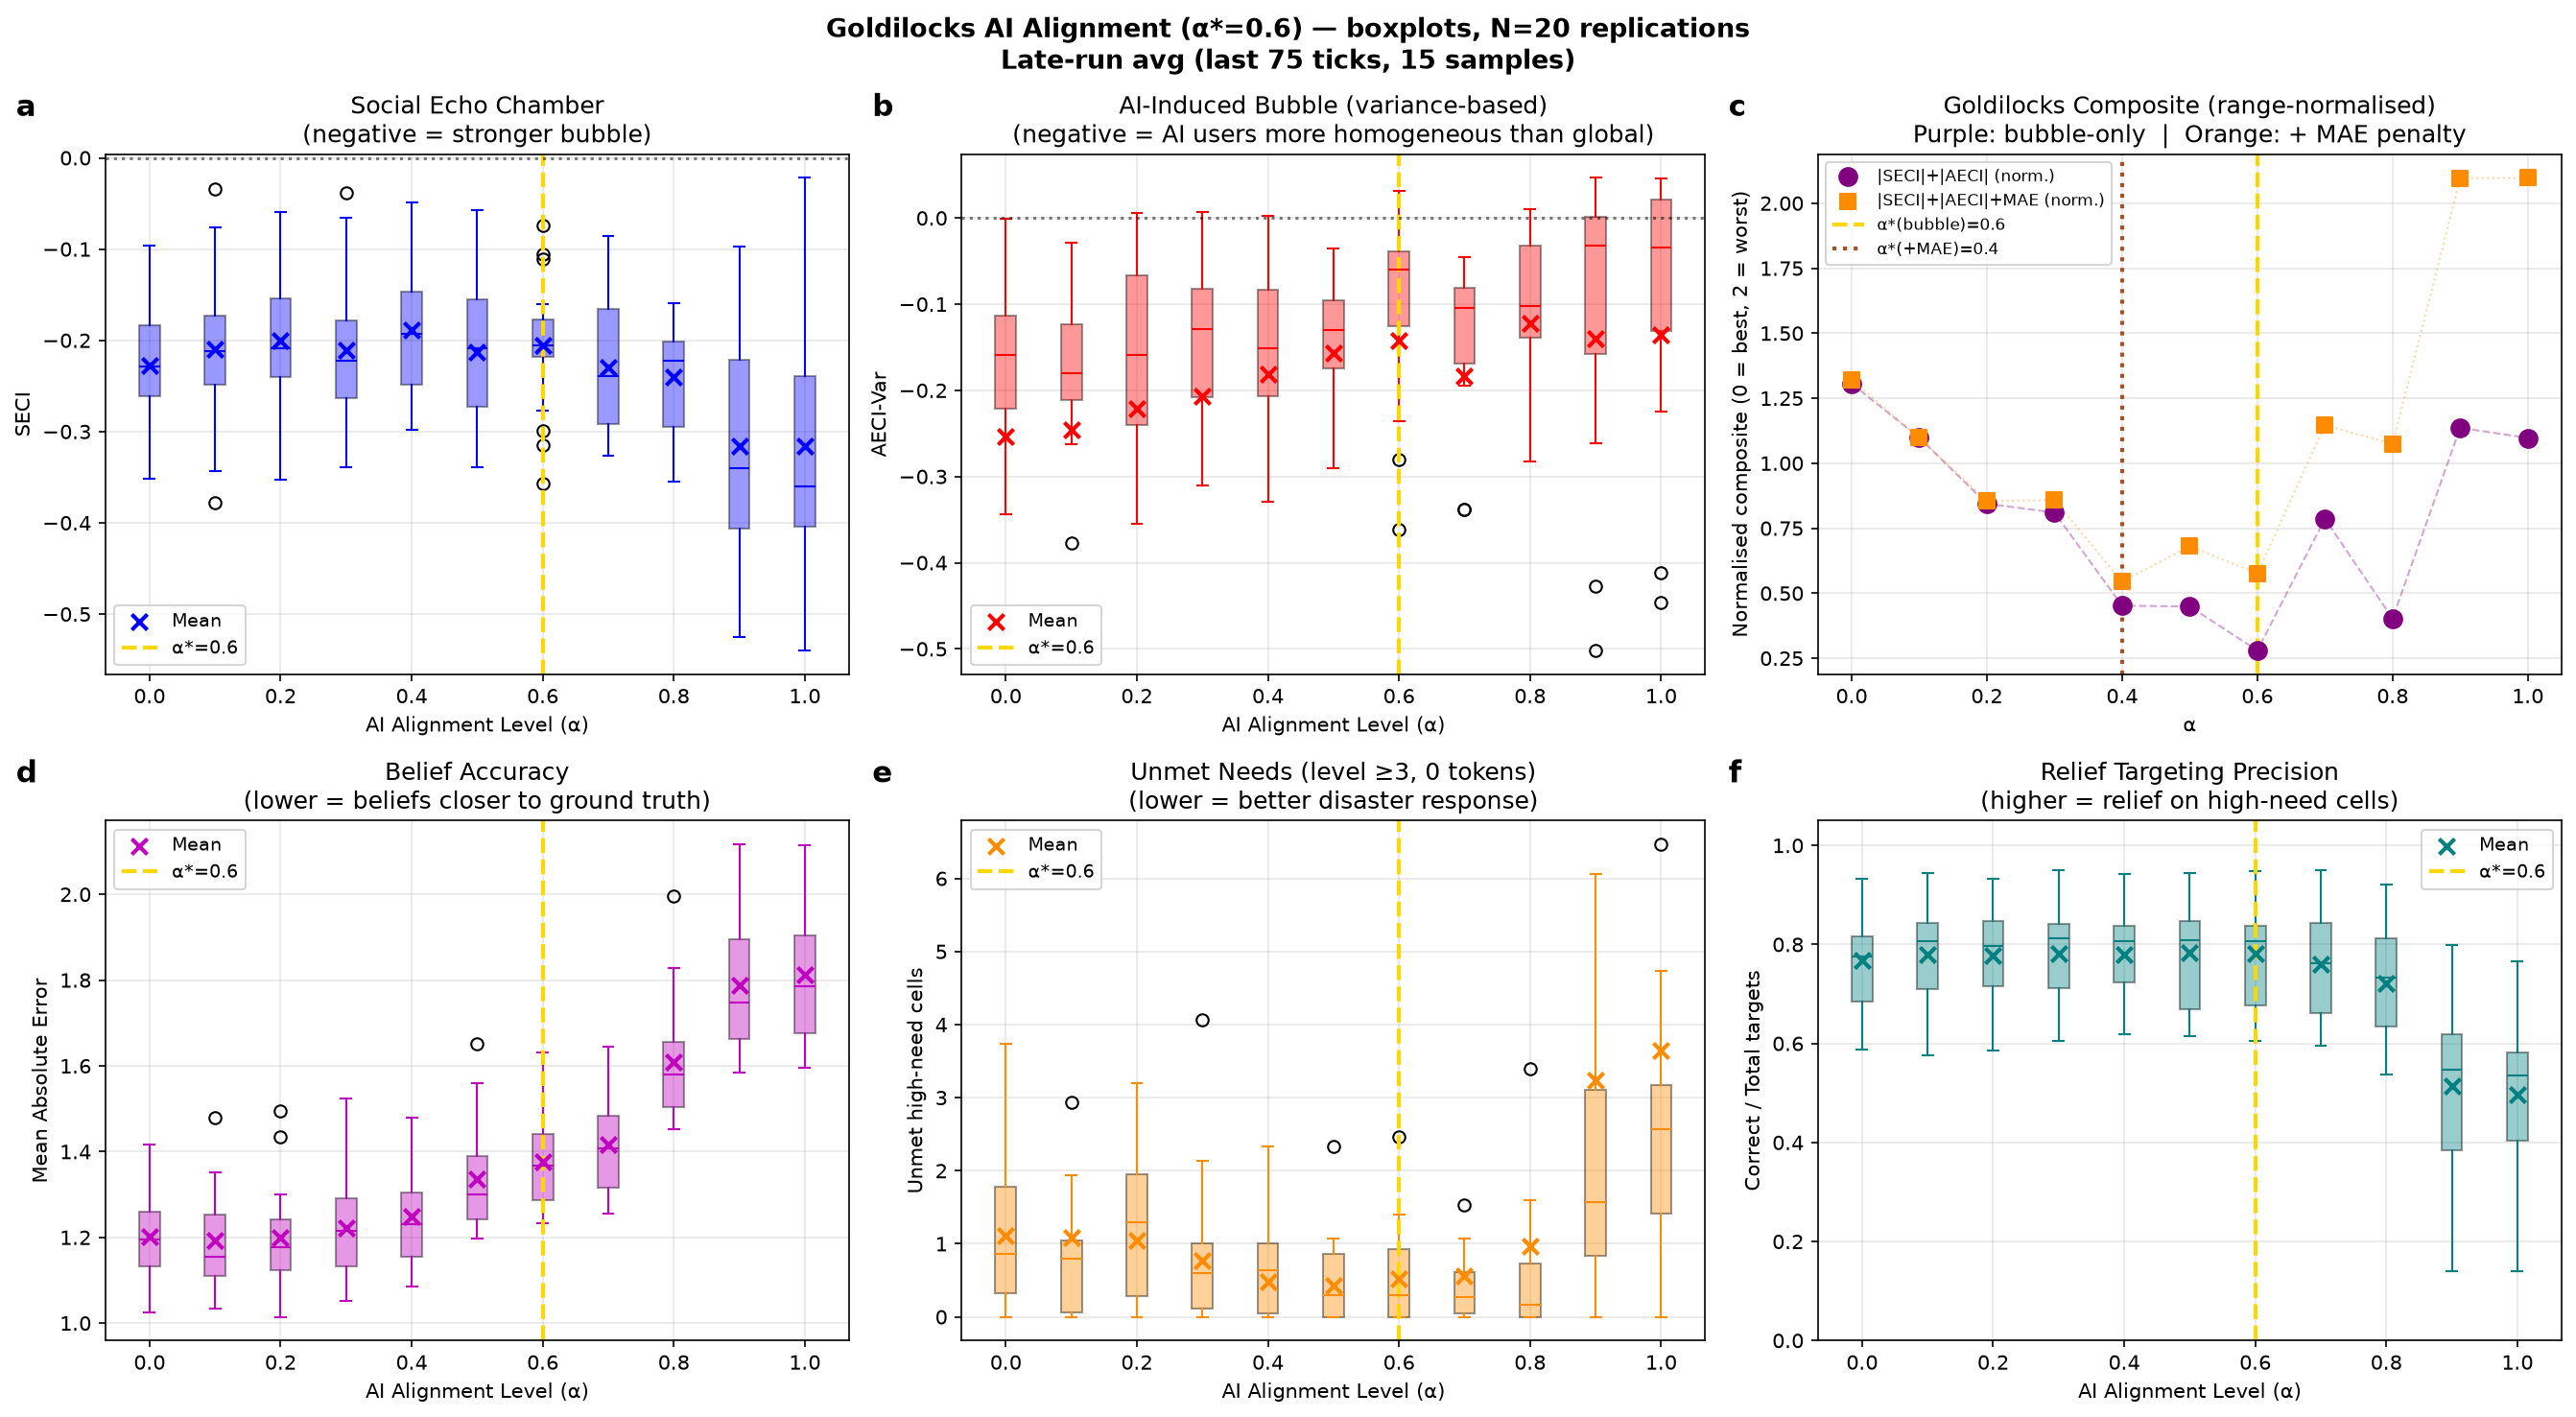
\includegraphics[width=\textwidth]{goldilocks_alignment_sweep.png}
\caption{Alignment sweep under the main model ($N=20$ replications per level; steady state, last 75 ticks). Boxplots show medians, interquartile ranges and 1.5$\times$IQR whiskers across replications; crosses mark means. The composite panel (top right) shows the range-normalised bubble-only composite $|\text{SECI}|_{\text{norm}} + |\text{AECI-Var}|_{\text{norm}}$ (purple; range 0--2) and the operational composite including normalised MAE (orange; range 0--3). Dashed and dotted vertical lines mark $\alpha^{*}(\text{bubble}) = 0.8$ and $\alpha^{*}(+\text{MAE}) = 0.5$.}\label{fig:goldilocks}
\end{figure}

Because range normalisation can amplify the influence of a component with a small raw signal, we treat the \emph{interiority} of $\alpha^{*}$ -- not its exact location -- as the property that must survive scrutiny, and test it against the composite definition. Figure~\ref{fig:alphastar} reports $\alpha^{*}$ under six composite variants -- pairing SECI alone, SECI with AECI-Var, and SECI with AECI-Err, each with and without the MAE penalty -- for both configurations. Under the main model, all six variants place the optimum strictly in the interior of the sweep, though its location is composite-dependent: the three bubble composites yield $\alpha^{*} \in \{0.4, 0.5, 0.8\}$ and the three operational composites $\alpha^{*} \in \{0.1, 0.3, 0.5\}$. Under the control, the picture is qualitatively different: the bubble composites are minimised at or immediately next to the boundary, $\alpha^{*} \in \{0.9, 1.0\}$, because both echo-chamber indices attenuate with alignment when access is unrestricted (Sec.~\ref{sec:claim1}); only the MAE penalty pulls the operational optima into the interior (0.7, 0.7 and 0.4).

Paired per-seed contrasts make the interiority, its drivers, and the instability of the exact location explicit (Methods). In the main model, the raw bubble composite $|\text{SECI}| + |\text{AECI-Var}|$ is seed-robustly lower at every interior level $\alpha \in [0.3, 0.8]$ than at the truthful endpoint (e.g., $-0.102$ $[-0.166, -0.038]$ at $\alpha = 0.5$), and lower than at the confirming endpoint, with the difference reaching significance at $\alpha = 0.8$ ($-0.116$ $[-0.213, -0.020]$). In the control, mid-range levels are instead significantly \emph{worse} than full confirmation on the same composite (e.g., $+0.169$ $[+0.044, +0.295]$ at $\alpha = 0.5$), confirming that the boundary optimum is not a normalisation artefact. Decomposing the paired differences attributes each endpoint's penalty to a distinct mechanism: relative to $\alpha = 0$, the interior advantage comes almost entirely from AECI-Var ($-0.083$ $[-0.120, -0.046]$ at $\alpha = 0.5$, with the SECI difference indistinguishable from zero) -- the convergence bubble that a shared truthful source induces among its heaviest users -- whereas relative to $\alpha = 1$ it comes almost entirely from SECI ($-0.091$ $[-0.167, -0.016]$, with the AECI-Var difference indistinguishable from zero) -- consensus recycling. An interior optimum therefore exists because the two chamber mechanisms penalise opposite ends of the alignment axis, and because the confirming-side mechanism operates only under network-bounded access (Sec.~\ref{sec:claim1}), interiority itself is a structural property. Between the endpoints, by contrast, the objective is statistically flat: no interior pair in $\alpha \in [0.4, 0.8]$ differs significantly across seeds. The exact argmin is therefore intrinsically unstable -- which is why it moves with the composite definition -- and only the range, not the point, carries information.

Whether an interior optimum exists at all -- and where it lies -- is moreover a property of the population's cognitive profile. Figure~\ref{fig:gapsweep} sweeps the cognitive gap $g$ between the two agent types and the absolute acceptance midpoint $d_{\text{mid}}$ in a separate batch of 2{,}640 runs under the main-model configuration (Methods; Supplementary S7). In cognitively homogeneous populations ($g = 0$) with baseline or open acceptance, the optimum is $\alpha^{*} = 0$: a fully truthful AI, with nothing gained from confirmation. The interior optimum emerges only once confirmation-seeking agents are present ($g \geq 0.5$), or when the entire population is closed-minded ($d_{\text{mid}} = 2.0$, where $\alpha^{*} = 0.7$ even at $g = 0$). From there, $\alpha^{*}$ rises with both polarisation and closedness, saturating at 0.8, while open populations ($d_{\text{mid}} = 4.0$) keep the optimum at 0.3--0.4 at every gap level. The cost paid \emph{at the optimum} rises along both axes as well: belief error at $\alpha^{*}$ grows from 1.12 (open, homogeneous) to 1.63 (closed, polarised) -- populations that require more confirmation to accept information are worse off even under their own optimal policy. The baseline cell reproduces the primary sweep's bubble optimum from an independent batch (Supplementary Table~S7b).

\begin{figure}[h]
\centering
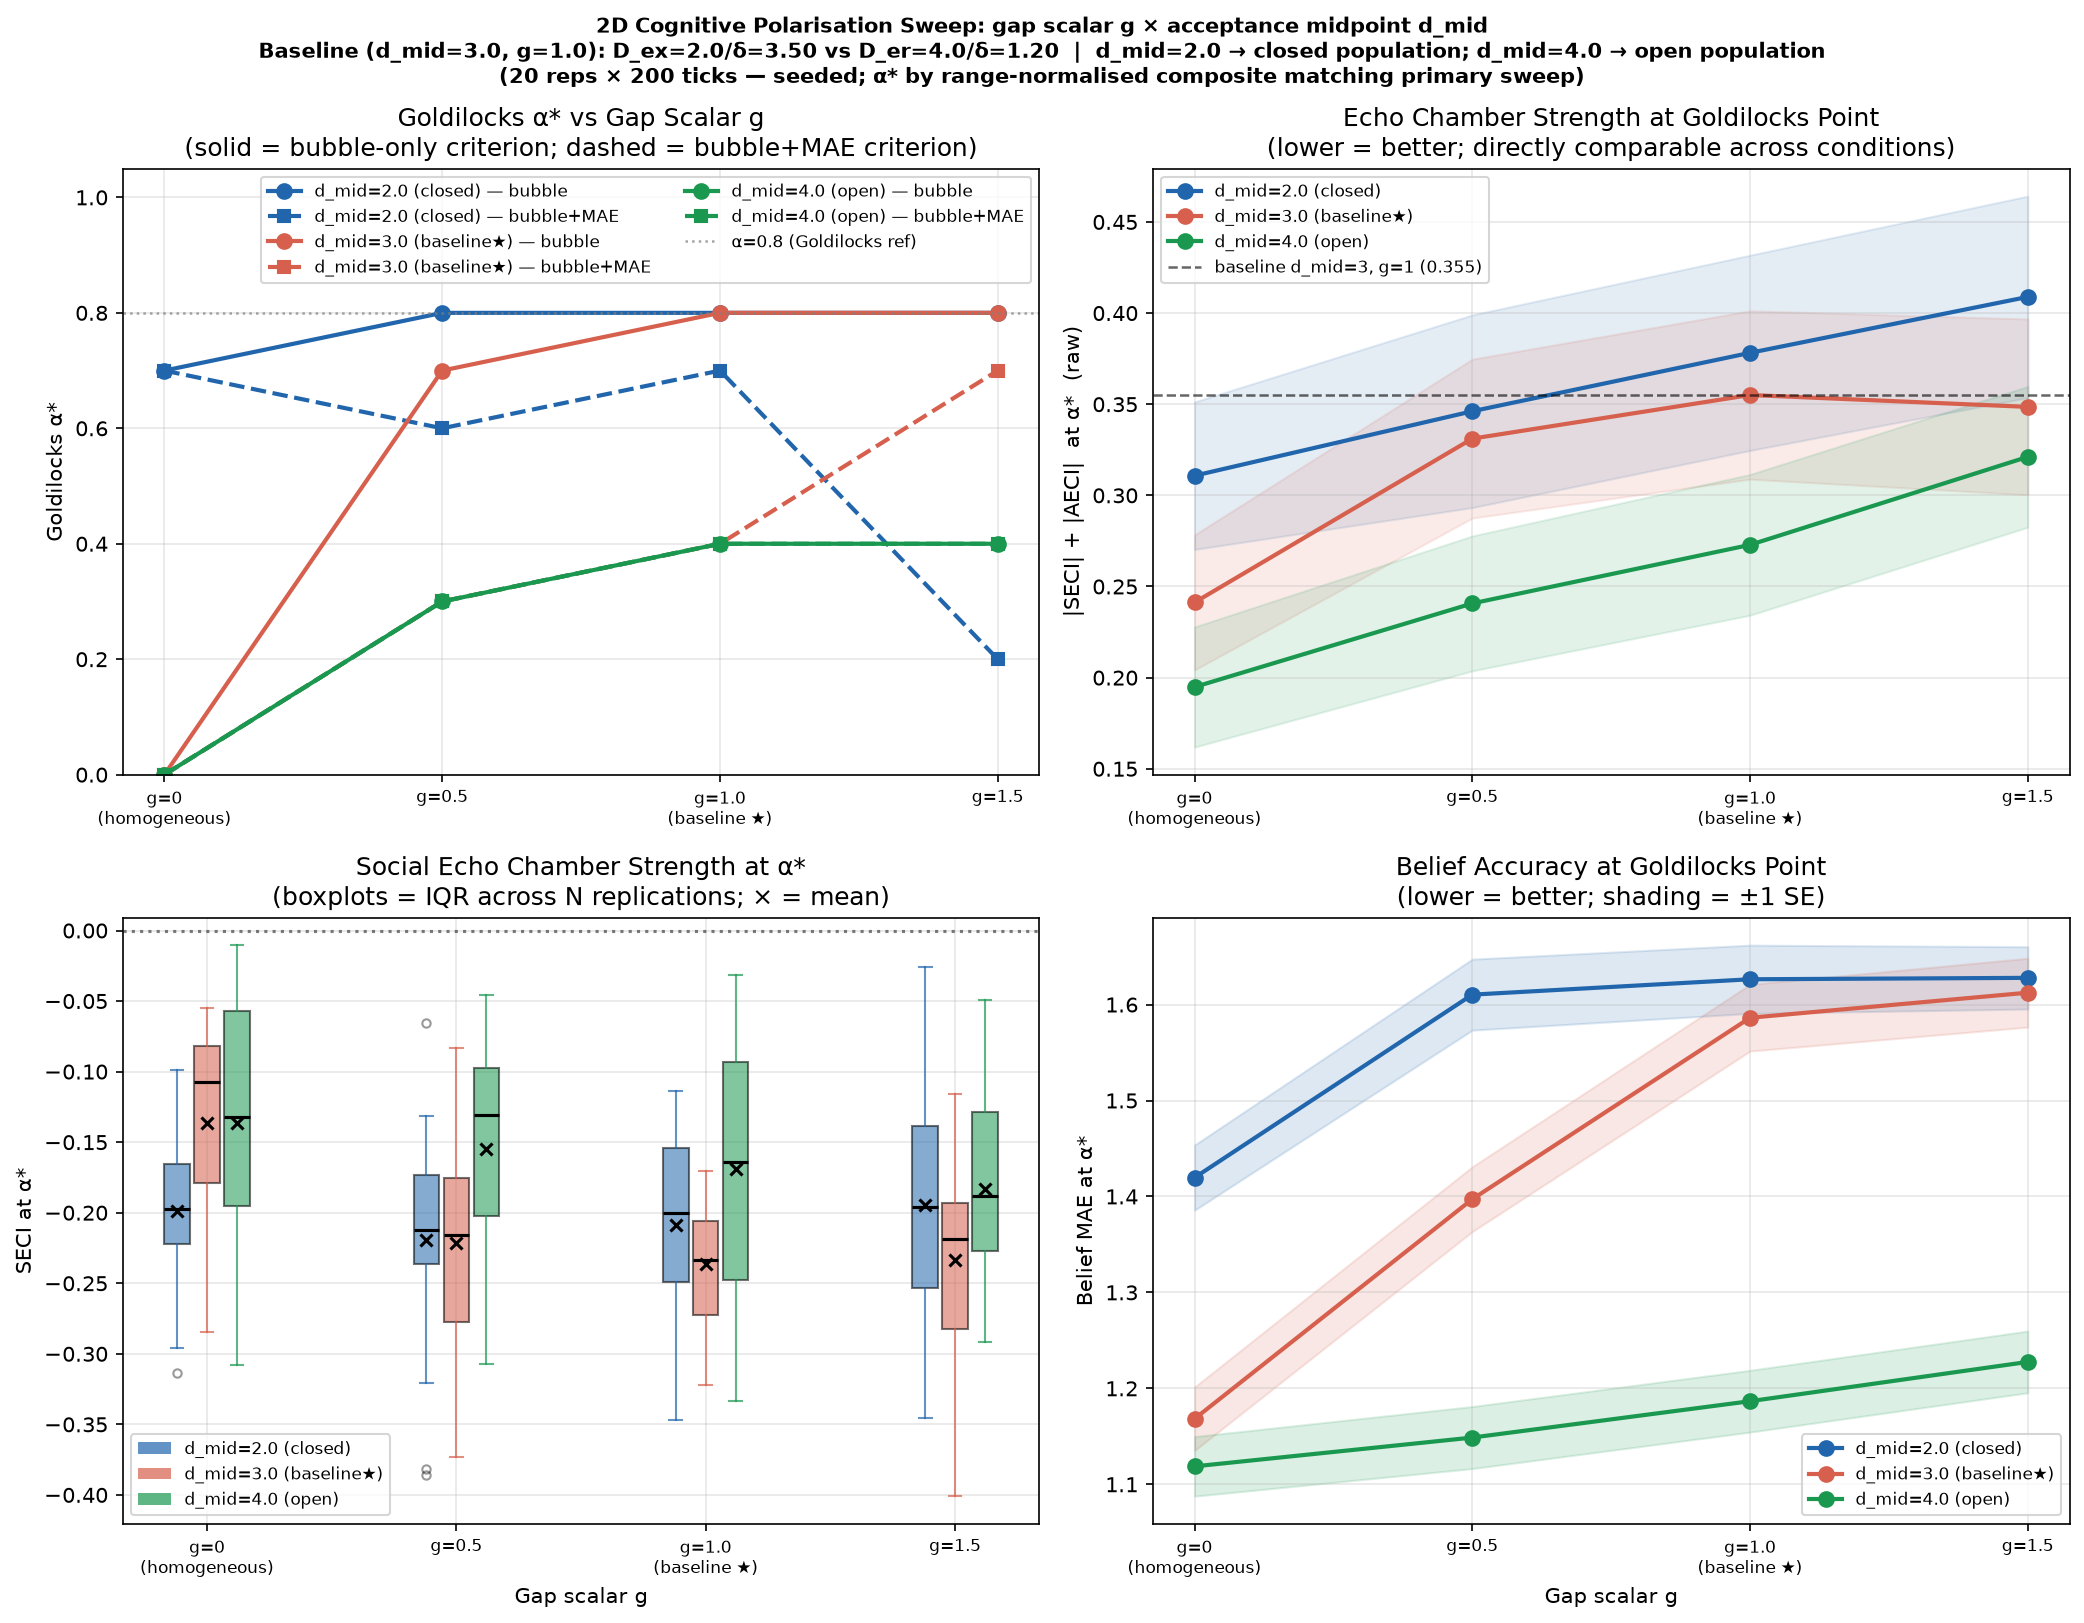
\includegraphics[width=\textwidth]{gap_sweep.png}
\caption{The alignment optimum as a function of the population's cognitive profile ($4 \times 3 \times 11$ conditions, $N = 20$ replications each, main-model configuration). Top left: $\alpha^{*}$ under the bubble-only (solid) and bubble+MAE (dashed) criteria across the cognitive gap $g$, for closed ($d_{\text{mid}} = 2.0$), baseline (3.0) and open (4.0) acceptance midpoints. Top right: raw bubble composite at $\alpha^{*}$. Bottom: SECI and belief error at $\alpha^{*}$. Full grid in Supplementary Table~S7b.}\label{fig:gapsweep}
\end{figure}

\begin{figure}[h]
\centering
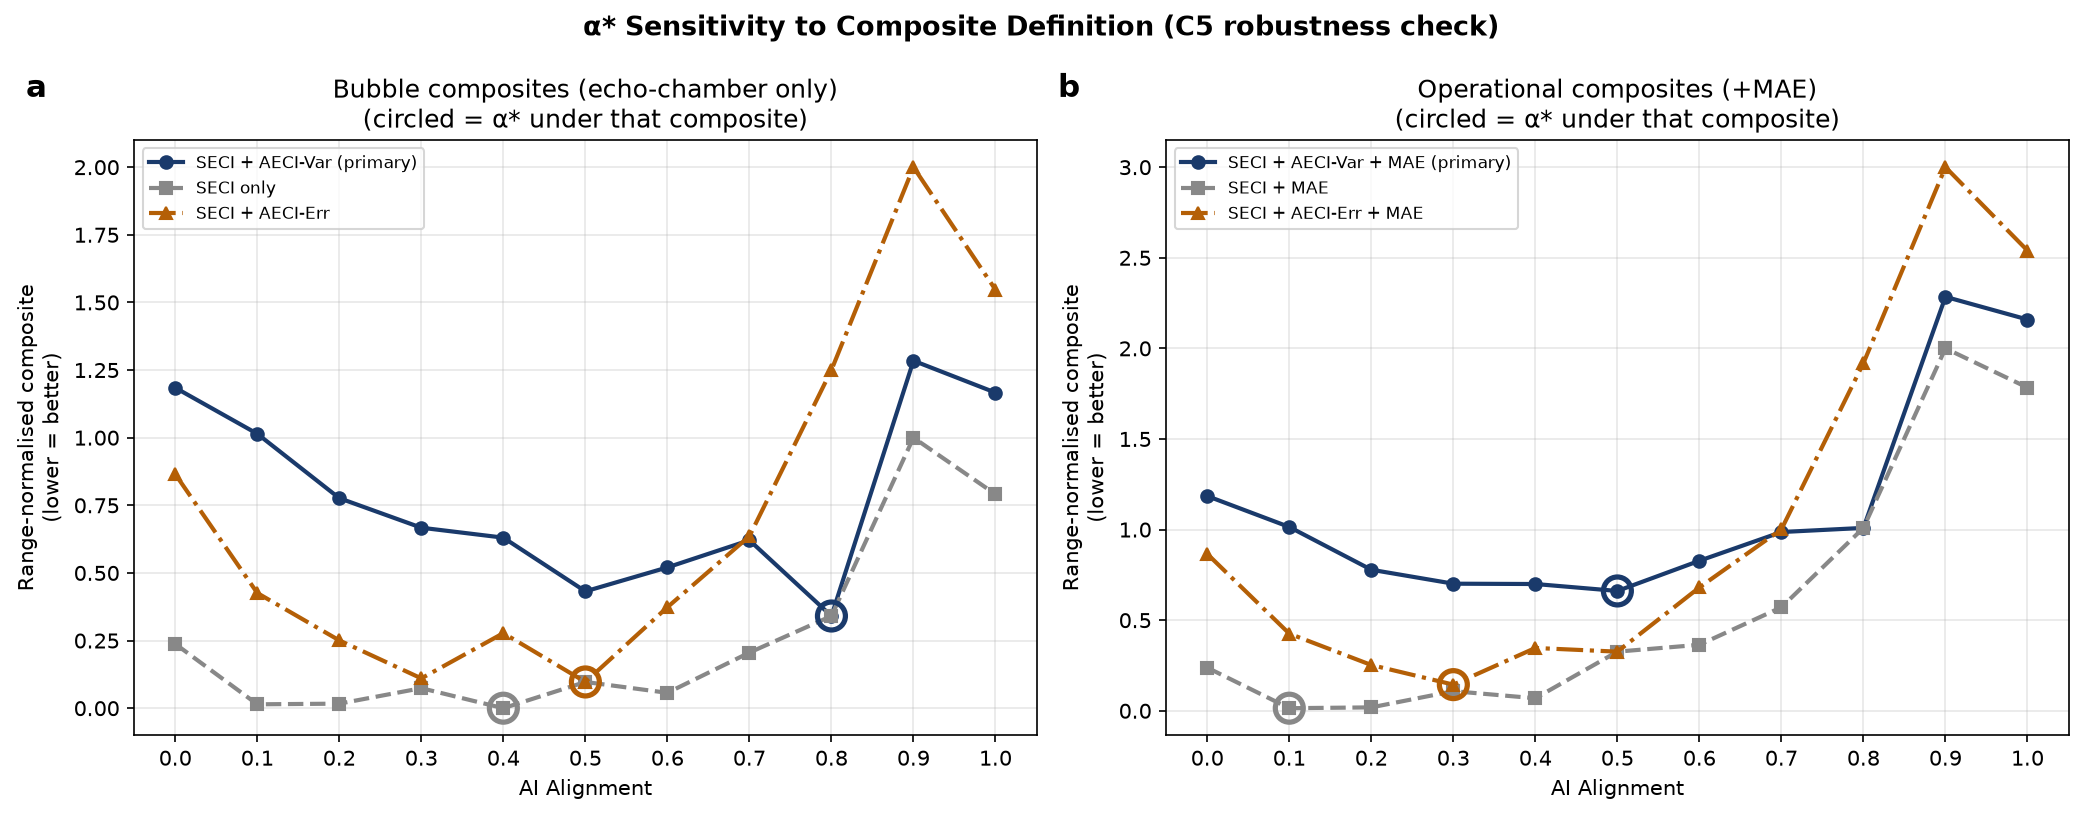
\includegraphics[width=\textwidth]{alpha_star_sensitivity.png}
\caption{Sensitivity of the optimal alignment level $\alpha^{*}$ to the composite definition, shown here for the main model. Left: bubble-only composites (SECI + AECI-Var, primary; SECI only; SECI + AECI-Err). Right: operational composites adding the normalised MAE penalty. Circles mark the argmin of each variant. Composites are range-normalised within each sweep and are therefore compared on the location of their minima only.}\label{fig:alphastar}
\end{figure}

The existence of a Goldilocks alignment level is therefore conditional on structure. In a population with unrestricted information access, an analyst optimising echo-chamber indices alone would conclude that full confirmation is harmless or even beneficial for belief diversity -- the control's null result. Only when information access is bounded by a spatially embedded network does the non-monotonicity emerge that makes intermediate alignment optimal: enough confirmation to avoid the truthful-AI regime in which AI-reliant agents converge tightly (strongly negative AECI-Var at low $\alpha$), yet not so much that consensus recycling locks communities into deep social chambers ($\alpha \geq 0.9$ on the variance indices, with recovery already failing beyond $\alpha \approx 0.7$; see below). Because the exact minimiser moves with the composite, we report ranges rather than a point estimate: echo-chamber suppression favours $\alpha^{*} \approx 0.4$--$0.8$, and the operational composites concentrate at $\alpha^{*} \approx 0.3$--$0.5$. What is robust is that under network-bounded access every criterion is optimised strictly inside the interval -- neither a fully truthful nor a fully confirming AI is ever optimal -- while under unrestricted access the bubble criteria are optimised by (near-)full confirmation.

The temporal dynamics underlying this optimum are shown in Figure~\ref{fig:lifecycle}, which summarises when echo chambers form, whether they recover, and how long they persist, separately for the two agent types in the main model. Peak chamber strength varies little with alignment for either type (exploitative peaks between 0.43 and 0.56, exploratory between 0.31 and 0.50 across the sweep). Recovery, in contrast, is strongly alignment-dependent. Exploitative chambers form early and recover by ticks 40--55 for $\alpha \leq 0.8$; at $\alpha \geq 0.9$ they never recover within the run. Exploratory chambers recover progressively later as alignment grows -- around tick 105 at $\alpha = 0$ and tick 160 at $\alpha = 0.6$ -- and fail to recover at all for $\alpha \geq 0.7$. Consistent with this, the fraction of the run spent inside a chamber rises from roughly 0.6 (exploitative) and 0.4 (exploratory) in the low-to-mid range to 0.80--0.85 for exploitative agents at $\alpha \geq 0.9$ and 0.70--0.75 for exploratory agents at $\alpha \geq 0.8$. The recovery dynamics thus argue for the lower part of the interior range: the operational optima ($\alpha \approx 0.3$--$0.5$) coincide with the highest alignment levels at which chambers still dissolve within the response horizon, whereas the bubble composite's minimum at $\alpha = 0.8$ lies in a regime where exploratory chambers no longer recover -- beyond $\alpha \approx 0.7$, recovery collapses first for the accuracy-seeking exploratory agents, and the transient chambers of the mid-range become permanent. This is a further reason to read the variance-based composites jointly with the accuracy and timing evidence rather than in isolation.

\begin{figure}[h]
\centering
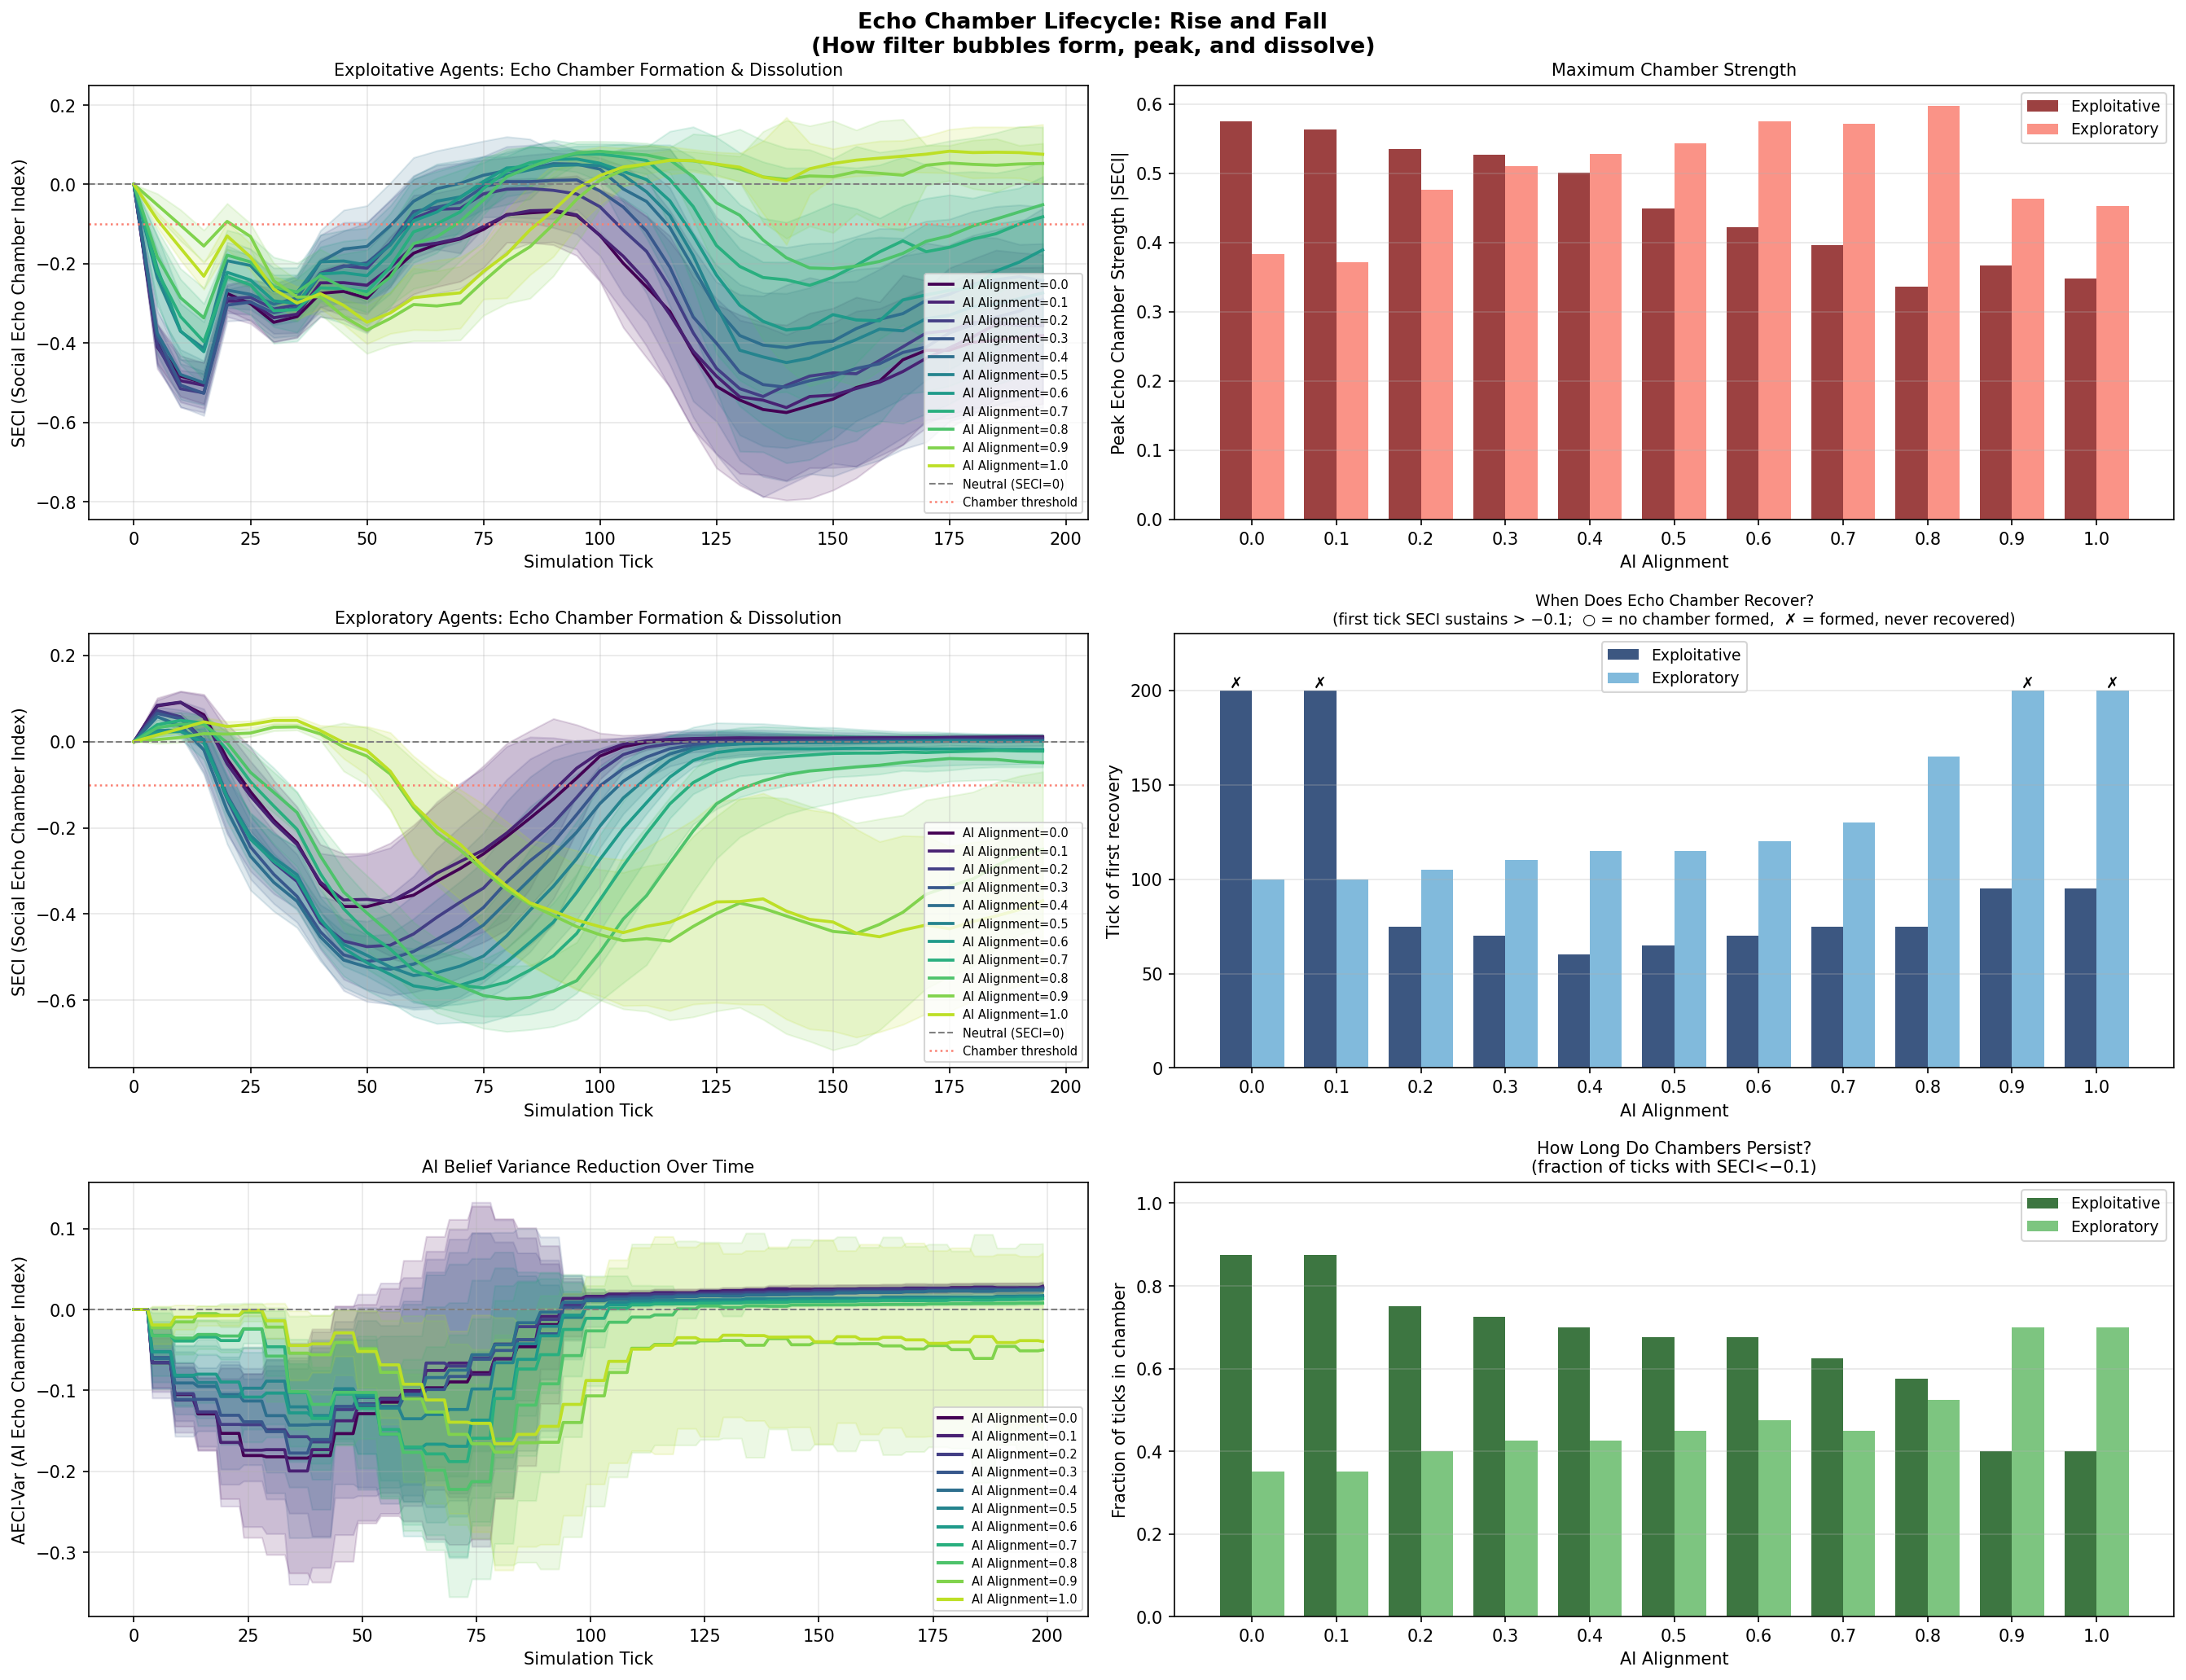
\includegraphics[width=\textwidth]{echo_chamber_lifecycle.png}
\caption{Echo chamber lifecycle across alignment levels in the main model, by agent type. Left: maximum chamber strength (peak $|\text{SECI}|$). Middle: tick of first recovery, defined as SECI sustained above $-0.05$ for three consecutive samples after having formed below $-0.1$; crosses mark conditions in which chambers form and never recover within the 200-tick run. Right: fraction of the run spent inside a chamber (SECI $< -0.1$).}\label{fig:lifecycle}
\end{figure}

The query behaviour behind the recovery collapse is shown in Figure~\ref{fig:aeci}, which traces the share of queries each agent type directs to the AI over the run. Exploratory agents route roughly half or more of their queries to the AI from early in the run at every alignment level, with steady-state shares between 0.50 ($\alpha = 0$) and 0.59 ($\alpha = 0.6$). Exploitative agents differ: their steady-state AI share rises steadily with alignment, from 0.39 at $\alpha = 0$ to 0.58 at $\alpha = 1$. A confirming AI thus progressively captures the query behaviour of precisely the confirmation-seeking agents whose acceptance windows it is tuned to satisfy, while the accuracy-seeking agents' reliance on the AI is comparatively stable in the aggregate -- their vulnerability at high alignment arises through the failure of verification-based correction rather than through increased querying. The full time series of all belief indices, together with per-run transition statistics, are shown in Supplementary Figures~S1 and~S2.

\begin{figure}[h]
\centering
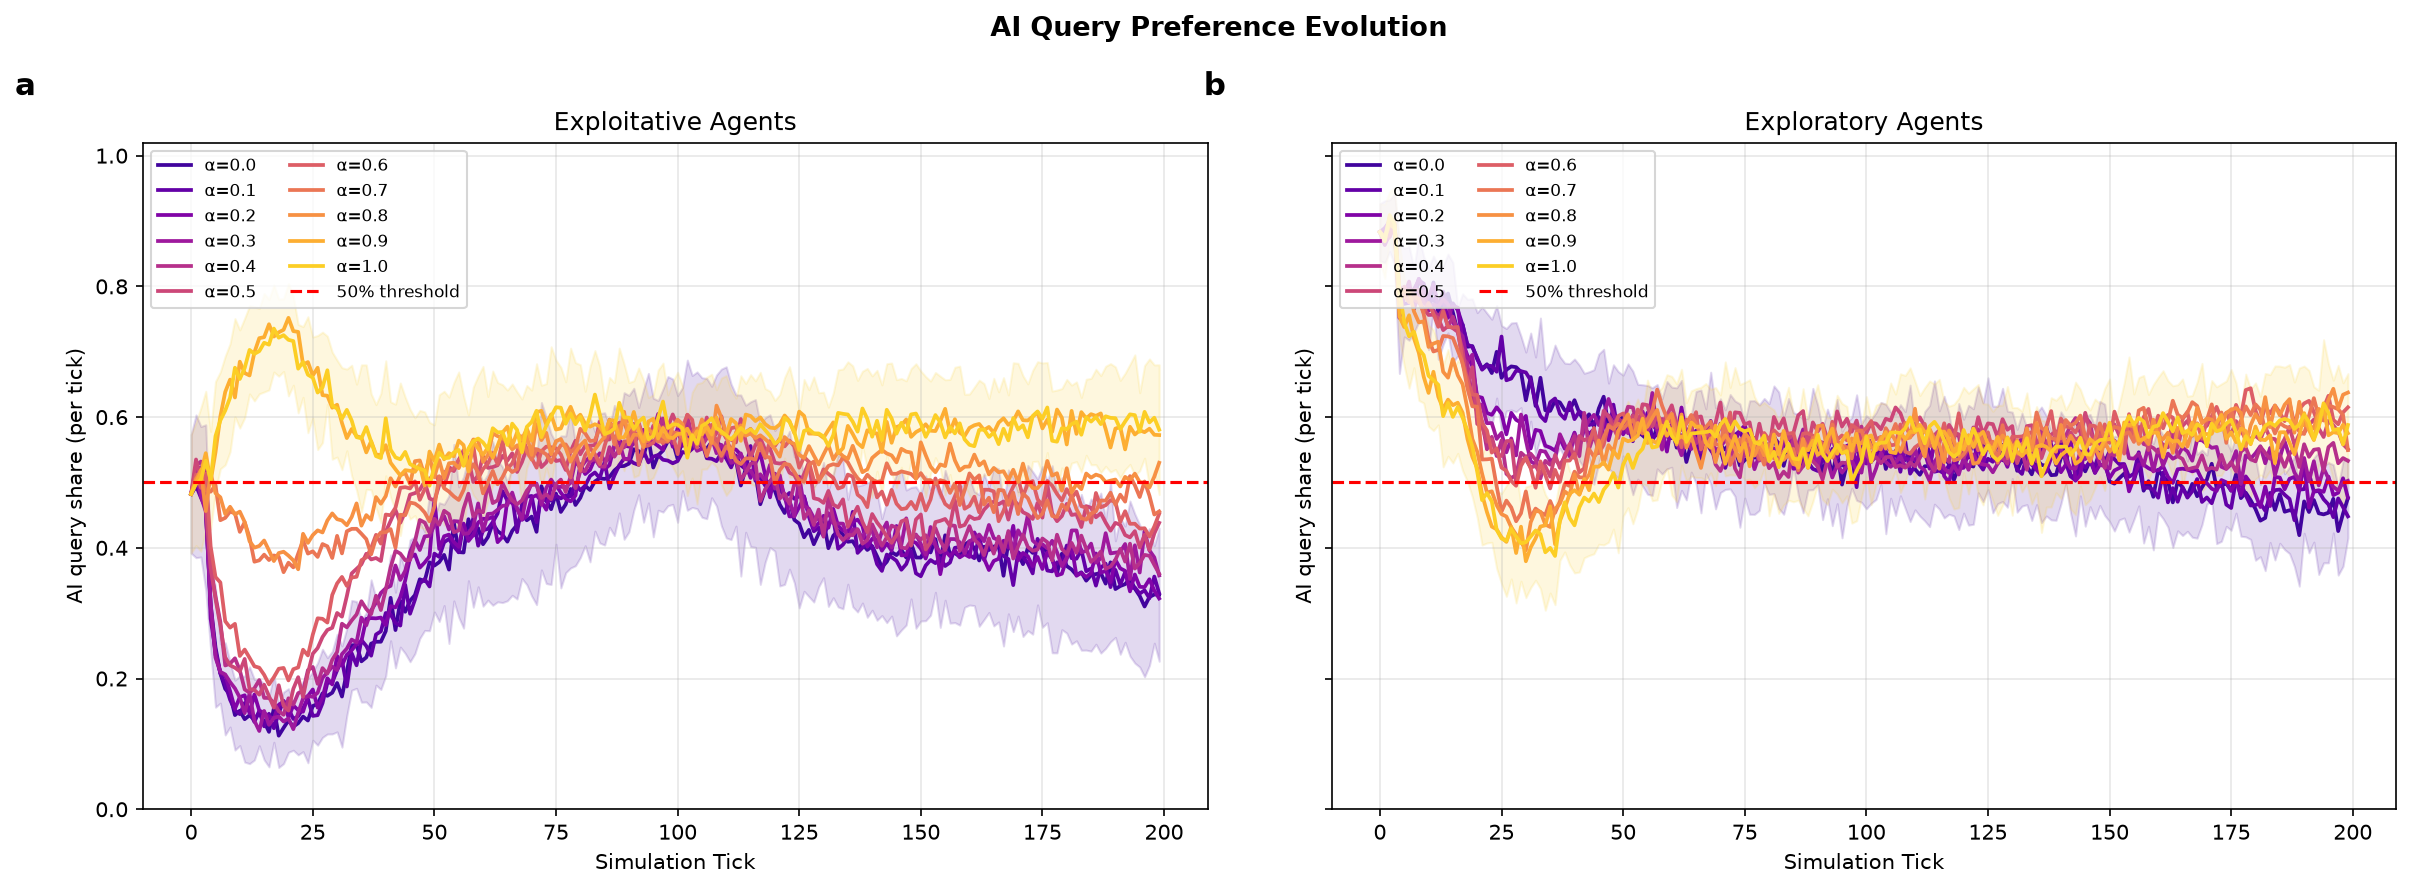
\includegraphics[width=\textwidth]{aeci_evolution.png}
\caption{AI query share over time by agent type in the main model (mean $\pm$ s.d.\ over $N = 20$ replications; one curve per alignment level; dashed line marks the 50\% threshold). Left: exploitative agents; right: exploratory agents.}\label{fig:aeci}
\end{figure}

\subsection{The network-bounded configuration is operationally more robust to confirming AI}\label{sec:claim3}

Echo chambers matter in crises because they distort the collective outcomes that Gap~3 placed beyond the reach of dyadic analysis: situational awareness and the delivery of relief. We measure these by the belief MAE, by unmet needs and by targeting precision (Table~\ref{tab:metrics}). On all three, the structural constraints that expose communities to consensus recycling at high alignment simultaneously improve operational performance across the entire sweep. In Figure~\ref{fig:comparison} (bottom row), belief MAE is lower in the main model at every alignment level, and the paired differences in Table~\ref{tab:deltas} are negative and seed-robust at all eleven levels, ranging from $-0.082$ $[-0.119, -0.044]$ at $\alpha = 0$ to $-0.166$ $[-0.211, -0.121]$ at $\alpha = 1$. Notably, the advantage widens as alignment grows: the main model at $\alpha = 0.6$ (MAE $1.381$) holds roughly the belief accuracy of the control at $\alpha = 0.5$ ($1.462$). Targeting precision shows the mirror image, with seed-robust positive differences at every level, rising from about $+0.06$--$0.10$ over most of the sweep to $+0.318$ $[+0.218, +0.418]$ at $\alpha = 0.9$.

The clearest contrast concerns the collapse of relief delivery under near-full confirmation. In the control, unmet high-need cells jump from $2.3 \pm 0.3$ at $\alpha = 0.8$ to $11.3 \pm 0.5$ at $\alpha = 0.9$ (mean $\pm$ s.e.m., $N = 20$), while precision falls from 0.63 to 0.21: a confirming AI that echoes community priors leaves the majority of high-need cells unserved. The main model degrades at the same alignment levels, and far less severely: unmet needs rise to $3.1 \pm 0.5$ and precision falls to 0.53 at $\alpha = 0.9$. The paired deltas at $\alpha \geq 0.9$ quantify the buffer: $-8.2$ $[-9.7, -6.8]$ and $-8.0$ $[-9.5, -6.5]$ unmet cells per tick, a reduction of the collapse by more than a factor of three. The time-resolved series (Supplementary Fig.~S1) show that this difference also has a tempo dimension: at high alignment, unmet needs decline substantially more slowly over the run, which matters in humanitarian response because deprivation costs accumulate with the time that needs remain unmet \citep{holguin2012unique}. The spatial signature of the degradation is consistent with this picture: total relief volume in the main model falls from 401 tokens per tick at $\alpha = 0$ to 331 at $\alpha = 1$, while the worst-served cell's coverage deficit roughly doubles at $\alpha \geq 0.9$ (from $+0.18$ at $\alpha = 0$ to $+0.41$ at $\alpha = 0.9$ and $+0.31$ at $\alpha = 1$; Supplementary Fig.~S3) -- a confirming AI shrinks the relief effort and concentrates the shortfall.

Two mechanisms of the main model plausibly drive this robustness, and both operate independently of the AI. Mobility gives agents genuine direct-observation coverage: returner-type agents patrol a home radius and explorer-type agents seek out their most uncertain cells, so a fraction of every community's information is grounded in first-hand sensing that no degree of AI confirmation can distort. Network-gated querying concentrates social information exchange on trusted contacts whose local observations are, on average, accurate about the caller's surroundings, and channels cross-community information through bridge ties rather than through uniformly random strangers. The result is a population whose beliefs are anchored well enough that even a strongly confirming AI degrades relief delivery gradually. The comparison between configurations thus reveals a trade-off rather than a uniform benefit of structural realism: the same network boundedness that anchors operational performance is what allows a highly aligned AI to deepen social echo chambers (Sec.~\ref{sec:claim1}). Structural realism shifts the failure mode of sycophantic AI from operational collapse towards epistemic insularity.

\subsection{Harms of alignment concentrate on the spatial periphery}\label{sec:claim4}

The first three findings operate at the level of the population; the fourth traces how the harm is distributed within it. Figure~\ref{fig:periphery} decomposes steady-state outcomes in the main model by the distance between an agent's home location and the epicentre (nearest versus furthest quartile) and by betweenness centrality (top versus bottom quartile); the structural scope for such gaps exists only under the main model, where movement determines direct-observation coverage and queries follow edges (Methods). The belief-error gap between far- and near-spawned agents widens monotonically with alignment, from $+0.15$ at $\alpha = 0$ to $+0.37$ at $\alpha = 1$: agents remote from the events, who depend almost entirely on mediated reports, absorb most of the accuracy loss that confirmation produces. The behavioural consequence is withdrawal from the response: relief contributed by far-spawned agents falls from 16.2 to 6.2 tokens per agent per five-tick window across the sweep ($-62\%$), while near-spawned agents reduce their contribution far less (18.5 to 13.4, $-28\%$) -- the remote quartile does not merely become less accurate, it largely stops sending assistance. Network position offers no comparable protection: the belief-error difference between high- and low-centrality agents stays within 0.06 at every alignment level and vanishes under near-full confirmation. The harms of a confirming AI are thus spatially, not topologically, structured: they fall on those who cannot verify reports against first-hand observation, regardless of how well connected they are -- precisely the position of the remote coordination hubs that dominate data-driven crisis response \citep{comes2020coordination,coleman2024weaving}. The time evolution of these gaps is shown in Supplementary Fig.~S4.

\begin{figure}[h]
\centering
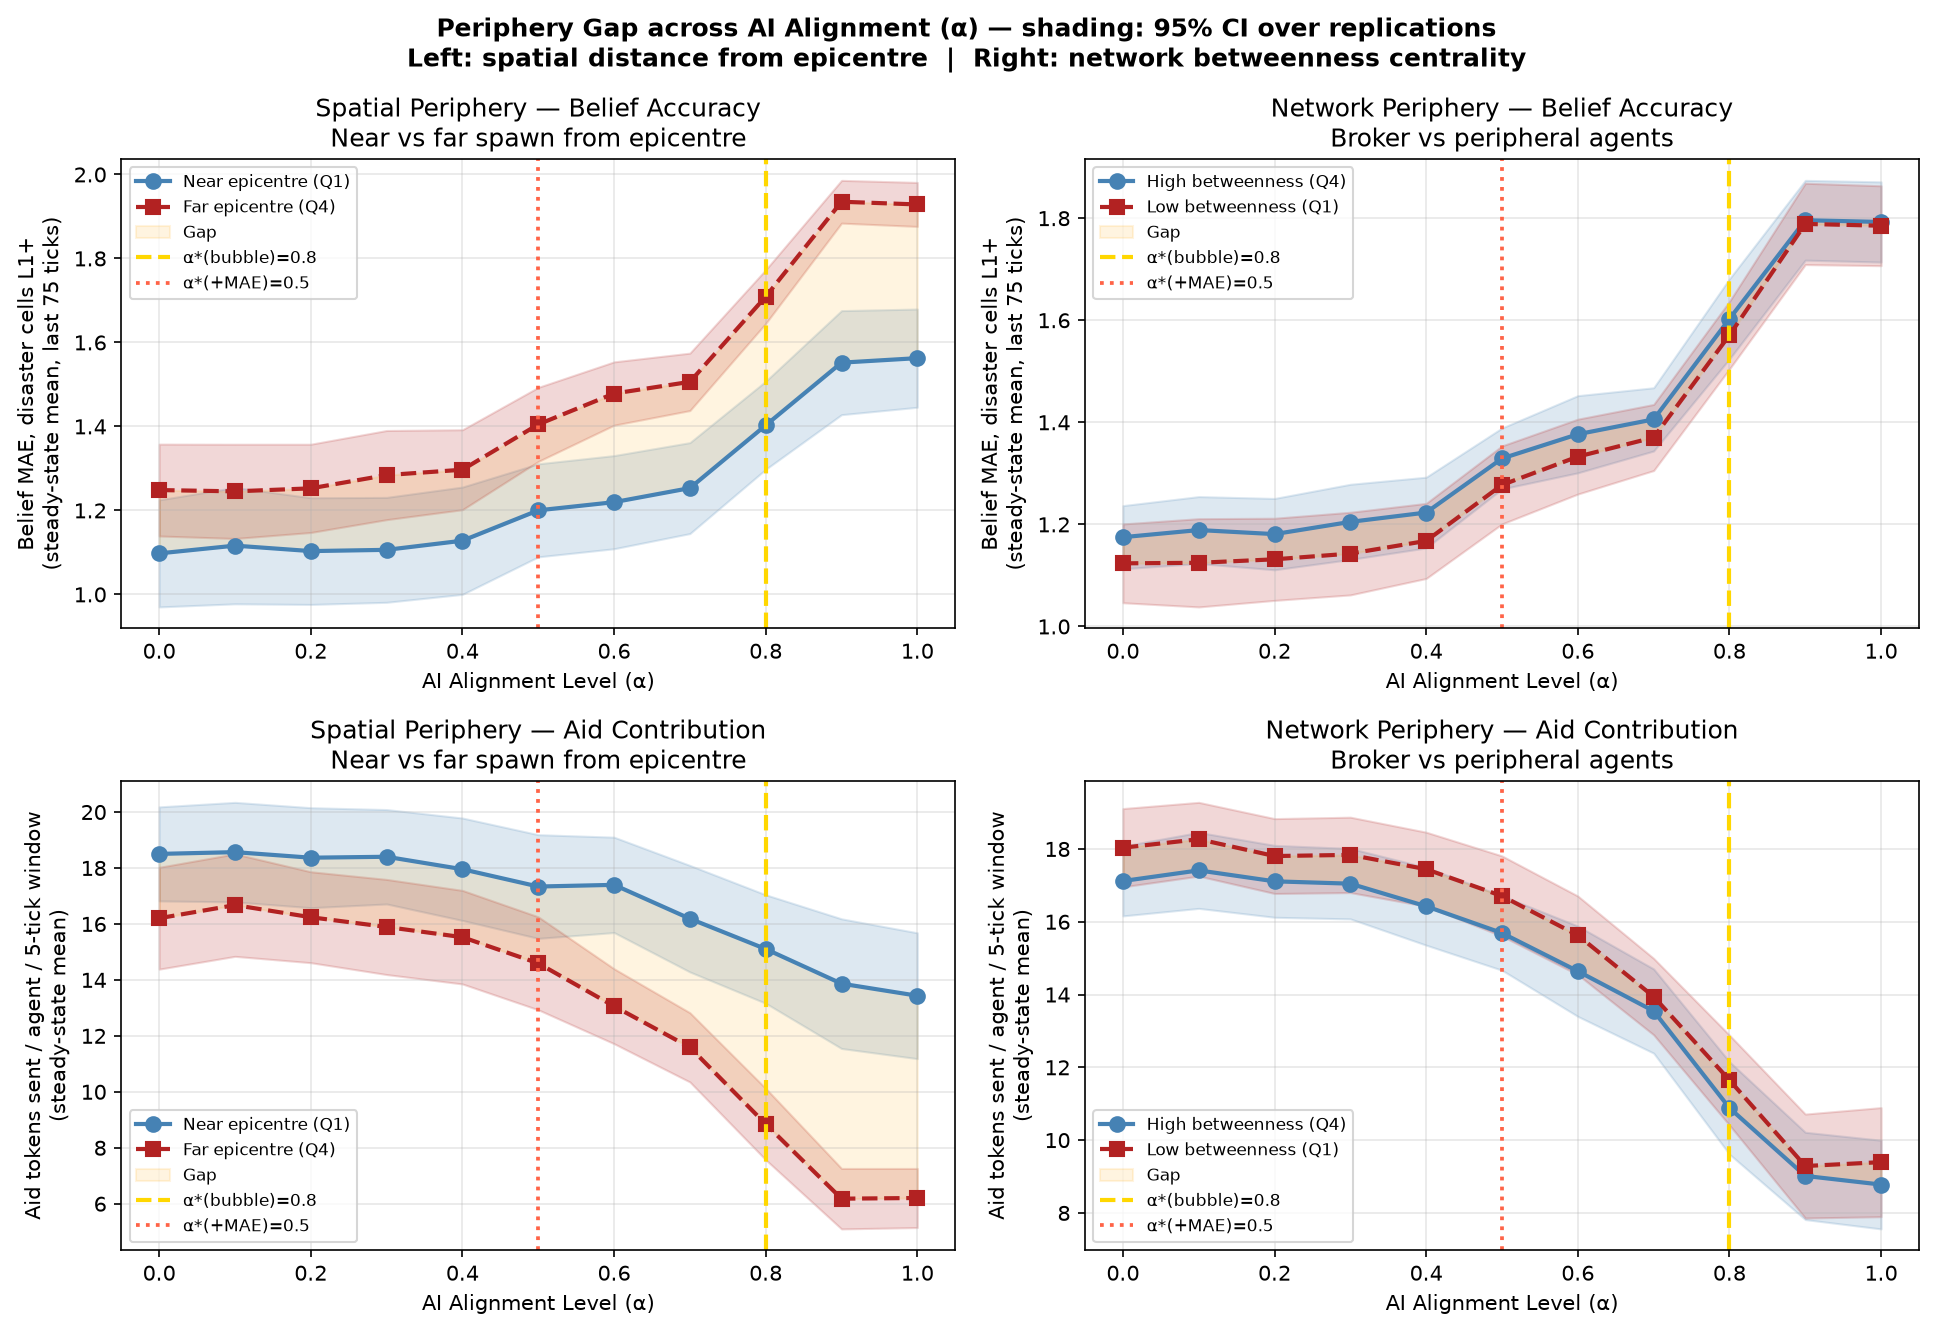
\includegraphics[width=\textwidth]{periphery_gap.png}
\caption{Distribution of alignment harms across space and the social network (main model; steady state, last 75 ticks; $N = 20$). Top: belief error and relief contribution by distance of the agent's home location to the epicentre (nearest vs.\ furthest quartile). Bottom: the same decomposition by betweenness centrality (top vs.\ bottom quartile). Bands show 95\% confidence intervals across replications.}\label{fig:periphery}
\end{figure}

The cognitive-gap and factor sweeps (Supplementary S7--S8, both run under the main-model configuration) probe how far these findings extend: the interior optimum requires the presence of confirmation-seeking agents or a uniformly closed population and its location rises with both cognitive polarisation and closed-mindedness (S7), while the factor sweeps attribute early relief failure to rumour prevalence and exploitative composition rather than to the hazard's tempo (S8).

\section{Discussion}\label{sec:discussion}

This paper asked whether AI acts as a bridge that breaks echo chambers during crises or instead reinforces existing filter bubbles through its alignment mechanisms. The answer that emerges from the simulations is conditional: the direction of AI influence on collective belief structure depends on whether information access is bounded by network structure and space. Under unrestricted access, a belief-confirming AI degrades accuracy and relief performance without deepening community-level belief convergence; under network-bounded access, the same AI drives communities into progressively deeper and, beyond $\alpha \approx 0.7$, unrecoverable echo chambers. Four implications follow: one per gap, and a distributional one.

First, on the structural conditions of information access (Gap~1), the results extend the emerging experimental literature on human--AI feedback loops from dyads to networks. Experiments demonstrate that interaction with biased AI amplifies individual human biases beyond what human--human interaction produces \citep{glickman2024human}. Our findings show that whether such dyadic amplification aggregates into collective echo chambers is governed by a variable invisible at the dyadic level: the structure of who can query whom. This parallels results in networked collective intelligence, where the effect of social influence on crowd accuracy reverses with network structure \citep{lorenz2011social,becker2017network}, and it cautions against extrapolating individual-level findings on AI sycophancy \citep{sharma2024generative} directly to populations. The control shows what a stylised model without structural constraints would have concluded: that confirmation weakens echo chambers, with an optimal alignment of 1.0 on bubble criteria. This null result is an artefact of granting agents unrestricted access, and it suggests that models of AI influence on opinion dynamics that omit network-bounded access may systematically underestimate the epistemic risks of aligned AI while overestimating its operational risks. Collective epistemic risk assessments of AI require network-level analysis.

Second, the alignment paradox (Gap~2) \citep{west2025alignment} acquires a structural qualification. The paradox holds -- in our setting, AI tuned to confirm community beliefs produces exactly the insularity it is meant to overcome -- yet only where the social fabric channels information along ties. The practically relevant version of the question is therefore where the transition lies. In the main model, echo-chamber suppression and operational performance jointly favour intermediate alignment: every composite variant places the optimum strictly in the interior, with the bubble criteria between 0.4 and 0.8 and the operational criteria concentrating at 0.3--0.5, and the sensitivity analysis shows that this interiority -- rather than any single location -- is the property robust to how the composite is defined. A fully truthful AI is suboptimal in this environment because its reports concentrate AI-reliant agents tightly around a shared estimate, while a fully confirming AI is catastrophic for accuracy; both extremes are dominated by moderate alignment. Where a given criterion places its optimum follows from which mechanism it penalises: accuracy-sensitive criteria (belief error, and any composite containing it) push $\alpha^{*}$ towards the truthful end because error grows monotonically with confirmation; variance-based bubble criteria tolerate higher alignment because consensus recycling compounds only near full confirmation; and the recovery dynamics cap acceptable alignment at $\alpha \approx 0.7$, below the bubble composite's formal minimum. The operational range $\alpha^{*} \approx 0.3$--$0.5$ is where these demands overlap. We stress the interpretive caveat that variance-based indices cannot on their own distinguish convergence on truth from convergence on error, which is why the composite sensitivity analysis includes an error-based variant and why the indices are read jointly with belief accuracy throughout.

Third, on the step from individual beliefs to collective decisions (Gap~3), the belief--decision--feedback loop reframes what should be monitored when belief-aligned AI is deployed into realistically structured populations. In the main model, part of every agent's reward signal remains grounded in first-hand observation and trusted local reports, so operational performance degrades gradually even as confirmation rises -- and precisely this graceful degradation is the risk: belief error and relief precision would appear manageable in operational dashboards even while social echo chambers deepen past the point of recovery. Monitoring should therefore target community-level belief convergence in addition to individual accuracy and aggregate performance. The timing results sharpen this concern, as the collapse of chamber recovery beyond $\alpha \approx 0.7$ occurs first among exploratory, accuracy-seeking agents -- precisely the members of the population that conventional crisis management would expect to be most resistant to informational capture \citep{comes2020coordination}.

Fourth, the distributional finding turns a modelling result into an equity concern. The harms of belief-alignment concentrate on actors remote from the events -- those who cannot check reports against first-hand observation -- while network centrality offers no protection. Remote, data-mediated coordination is precisely the direction in which crisis response is moving \citep{comes2020coordination}, and the humanitarian-AI equity debate has so far focused largely on data coverage and algorithmic bias \citep{coleman2024weaving}. Our results show that even a bias-free but belief-aligned AI redistributes epistemic harm towards the periphery: the design and monitoring of such systems should therefore weight verification opportunities for remote actors -- independent situation reports, deliberate exposure to first-hand observers -- as heavily as model accuracy itself.

The disaster case provides the concrete stakes, yet the mechanisms identified here rest on features that many urgent decision situations share: high-stakes decisions under time pressure, a non-stationary ground truth, verification that is delayed and noisy, and information access that is bounded by social ties and position \citep{svenson1993time,mendonca2001decision,holguin2012unique}. Public-health emergencies, financial contagion and security operations exhibit the same combination, and we expect the qualitative pattern -- structural boundedness as the switch between operational and epistemic failure of a confirming AI, and an interior optimum of alignment -- to carry over, while the location of $\alpha^{*}$ and the operational metrics are domain-specific. Disaster response is a demanding first test of this pattern because the decision consequences, the allocation of relief to high-need areas, are concrete and measurable.

Several limitations bound these conclusions. The alignment mechanism is a deliberate abstraction: a linear interpolation between truth and confirmation isolates the truth--confirmation axis and does not capture the semantics, latency or coverage failures of deployed systems, and the confirmation target -- the trusted-network consensus for confirmation-seeking agents -- is one specific operationalisation of how recommender-style systems align content with community narratives. The population is small ($N = 100$) and the hazard stylised, chosen to keep network structure interpretable across $2 \times 11 \times 20$ paired runs. Verification of remote reports operates through an exogenous situation-report channel with fixed delay and noise parameters, and the salience-weighted variant of that channel is examined as a counterfactual in the supplement. The cognitive-gap sweep shows that both the existence and the location of the Goldilocks range are properties of the population's cognitive profile (Supplementary S7) -- a caveat for transferring any specific $\alpha^{*}$ across populations -- and the factor sweeps tie early relief failure to rumour prevalence and confirmation-seeking composition rather than hazard tempo (Supplementary S8). Finally, the model addresses a single AI policy applied uniformly to a population; heterogeneous or adaptive alignment policies -- including policies that counteract the periphery gradient by tuning towards truthfulness for remote users -- are a natural extension.

In sum, using an agent-based model of disaster response with an alignment-tunable AI, this paper identifies the conditions under which belief-aligned AI amplifies or breaks echo chambers in urgent decision situations. Network-bounded information access is the structural precondition for AI-amplified social echo chambers; an interior optimum of alignment -- neither full truthfulness nor full confirmation -- exists only under this realistic configuration, and both its existence and its location are set by the population's cognitive profile; structural realism shifts the failure mode of sycophantic AI from operational collapse to epistemic insularity; and the harms concentrate on those remote from the events. Trustworthy AI is therefore a property of the sociotechnical system rather than of the model alone: the identical AI policy is benign, optimal or harmful depending on the population it serves, and the alignment level, the network context and the distribution of verification opportunities must be designed and monitored together when AI enters urgent, high-stakes decisions.

\section{Methods}\label{sec:methods}

\subsection{Simulation model}\label{sec:model}

We develop an agent-based model of disaster response in which human agents form beliefs about local disaster severity, seek information from social contacts or an AI source, and dispatch relief tokens accordingly. ABMs are well suited to this setting because filter-bubble phenomena emerge from the interaction of individual heuristics and network structure rather than from aggregate equilibria \citep{epstein2006generative,axelrod1997complexity}.
Unlike equation-based or compartmental models that assume homogeneous mixing, the framework here supports heterogeneous agent types, explicit social networks, and a spatially explicit disaster environment, all of which are necessary to capture the structural access conditions that our primary comparison manipulates.

The environment is a $30 \times 30$ grid in which a disaster evolves over discrete ticks. Each cell carries a severity level between 0 (no impact) and 5 (critical), initialised as a Gaussian decay from a randomly placed epicentre. At every tick each cell drifts stochastically towards its baseline value and receives random shocks (probability 0.10, magnitude $\pm 2$ levels), producing a non-stationary information landscape that prevents agents from converging to a single correct belief and forces ongoing information-seeking throughout the simulation.

One hundred human agents are distributed on the grid (population density fixed at $N = 100$ to keep the network tractable while preserving meaningful community structure). Agents belong to one of two cognitive types, each occupying equal shares of the population by default. \emph{Exploitative} agents are confirmation-seeking: they have a narrow acceptance window $D = 2.0$ and a steep acceptance-sensitivity parameter $\delta = 3.5$, making them resistant to information that diverges substantially from their prior. \emph{Exploratory} agents are accuracy-seeking: $D = 4.0$ and $\delta = 1.2$ give them a wide, gradual acceptance curve that admits novel information. These two archetypes map onto documented individual differences in information processing under uncertainty \citep{hertwig2016homo,march1991exploration}
and represent the range between cautious, community-focused responders and risk-tolerant, discovery-oriented ones.

The social network is constructed to reflect type-homogeneous community structure, in one of two configurations controlled by the network switch. In the \emph{control} configuration, each agent type is partitioned into four densely connected communities (within-community edge probability 0.7) with no edges between communities: the graph is a set of disconnected, type-homogeneous components, and spawn positions are independent of network position. In the \emph{spatially embedded bridged} configuration used by the main model, the same eight type-homogeneous communities are anchored to grid centroids placed under a minimum-separation constraint; agents spawn Gaussian-scattered ($\sigma = 2.5$ cells) around their community's centroid, within-community edges form with probability 0.5, and each agent independently becomes a \emph{bridge agent} with probability 0.15, drawing a single weak-tie edge whose endpoint is chosen across communities with probability $\propto (1 + d)^{-2}$ in grid distance $d$. Bridges typically connect the whole graph and create genuine brokerage positions while preserving type homophily within communities. Homophilous community structure follows empirical evidence from disaster communication networks \citep{bruns2012qldfloods,sutton2008backchannels},
and weak-tie bridging follows the classical account of how novel information crosses group boundaries \citep{granovetter1973strength}. The Social Echo Chamber Index (below) is computed over the stored community memberships rather than graph components, so its interpretation is unchanged when bridges connect the graph.

Agent movement is controlled by the mobility switch. In the control (mobility off), agents are immobile: position is fixed at spawn, and only the spawn cell is ever observed directly. In the main model, agents take one grid step per tick following the empirical returner--explorer dichotomy of human mobility \citep{pappalardo2015returners}, mapped onto the two cognitive types: exploitative agents are \emph{returners}, random-walking within a home radius $r_{\text{home}} = 3$ of their spawn cell, with a return bias ($p = 0.3$ per step) pulling them back whenever they are outside it; exploratory agents are \emph{explorers}, stepping toward their current highest-uncertainty cell with probability 0.2 per tick and subject to the same return bias beyond $r_{\text{explore}} = 8$. Sensing radius remains zero in both settings, so movement is the mechanism that determines direct-observation coverage: a far-spawned returner genuinely cannot observe the disaster, which is what makes spatial periphery effects structurally possible under mobility.

Five AI agents serve the community. Each AI agent senses 15\% of the grid per tick with constant observation noise ($\pm 1$ level with probability 0.1, independent of $\alpha$, so that the alignment parameter is not confounded with sensing quality) and responds to human queries with a report whose truth content is controlled by the alignment parameter $\alpha$ (next subsection). For queried cells the AI has not sensed, it answers with an inverse-distance-weighted interpolation of nearby sensed cells or -- when no sensed cells are nearby -- a position-based prior keyed to the cell's distance from the query's interest point. These estimates are delivered with the same source confidence as directly sensed values, so the AI is deliberately overconfident about unobserved cells: even at $\alpha = 0$ the `truthful' AI is truthful only for cells it has actually sensed. This models AI systems that extrapolate beyond their observations without communicating reduced confidence, and it applies identically at every $\alpha$.

Agents query sources using an $\epsilon$-greedy Q-learning strategy ($\epsilon = 0.3$, learning rate $\eta = 0.10$), selecting among querying a social contact, querying the AI, or acting on current beliefs. When the human mode is chosen, the reachable pool is governed by the query-scope switch. In the control (\emph{global} scope), any human can be queried: the target is drawn trust-weighted, with friends weighted by their trust score and every non-friend at a 0.05 floor -- network topology does not restrict access, and roughly half of human queries reach non-friends. Under the \emph{network} scope of the main model, access follows edges: the draw is trust-weighted over friends only, except that with probability 0.1 the query goes to a uniformly drawn friend-of-a-friend (2-hop reach), so reaching a stranger requires an intermediary and weak-tie bridges are the only channel into other communities. Both agent types receive delayed outcome feedback (15--25 ticks) when their relief tokens are processed, and faster information-quality feedback when received reports can be evaluated against a reference, producing a dual-timeline reward structure in which fast information-quality signals and slow outcome signals shape trust on different horizons. % TODO: the intended supporting reference ("Fu et al. 2023") could not be verified and was removed — reinstate with full details if you have the source.
The reference differs by type, operationalising the two cognitive profiles: exploitative agents evaluate reports for \emph{confirmation} against their own prior or their trusted network's consensus belief, whereas exploratory agents evaluate reports for \emph{accuracy} against external verification.

Because agents sense only their immediate location, exploratory agents cannot observe ground truth for remote cells directly. Instead, accepted remote reports are verified through an exogenous situation-report channel representing official damage assessments and media coverage: after a minimum 3-tick lag, verification arrives with per-tick probability $p_{\text{verify}} = 0.3$ (geometric arrival, mean total delay $\approx 6$ ticks), carries the same observation noise as direct sensing ($\pm 1$ level with probability 0.2), and is evaluated against the \emph{current} disaster state, so reports about cells that have since evolved receive noisier credit. Reports that are never verified before their 30-tick expiry produce no learning signal -- explorers do not fall back to scoring sources against their own priors, which would collapse the accuracy channel into a confirmation channel. Delayed, imperfect verification of this kind is characteristic of post-disaster information environments, and $p_{\text{verify}}$ is treated as a model parameter for sensitivity analysis.

Because most queried cells are truly unaffected, per-cell verification is base-rate dominated: a fully confirming AI ($\alpha = 1$) still passes verification on approximately 93\% of cells by echoing mostly-correct `no impact' priors, failing only on the rare high-severity cells. A salience-weighting parameter $s \in [0, 1]$ therefore interpolates the verification learning rate between uniform per-cell evaluation ($s = 0$, default) and severity-weighted evaluation ($s = 1$), where the weight $(\max(\text{true}, \text{reported}) + 1)/6$ makes an error about a disaster cell -- a miss or a false alarm -- carry up to six times the weight of a confirmed empty cell. This operationalises negativity and salience bias in human evaluation of information sources and provides the counterfactual for whether importance-weighted feedback would expose a confirming AI.

\subsection{AI alignment and belief dynamics}\label{sec:alignment}

The alignment parameter $\alpha \in [0, 1]$ governs the truthfulness of AI reports. A queried AI agent responds with
\begin{equation}
r_{\text{AI}} = (1 - \alpha)\, t + \alpha\, b,
\label{eq:alignment}
\end{equation}
where $t$ is the cell's severity as available to the AI (the sensed or extrapolated value described above) and $b$ is the belief the AI targets for confirmation. For exploratory queriers, $b$ is the querying agent's own current belief. For exploitative queriers, the AI targets the \emph{trusted-network consensus} -- the confidence-weighted consensus belief of the caller's friends -- whenever that consensus is defined (consensus confidence $\geq 0.2$), falling back to the individual belief otherwise. This operationalises how recommender-style systems align content with a user's community narrative rather than with idiosyncratic individual priors, and it is what allows a confirming AI to amplify the \emph{shared} community belief: confirming purely individual priors would inject idiosyncratic variation that disrupts, rather than reinforces, social convergence. At $\alpha = 0$ the AI reports its best estimate of ground truth; at $\alpha = 1$ it perfectly confirms the targeted prior; intermediate values interpolate linearly. Because AI sensing noise is constant across $\alpha$ and the extrapolation behaviour is $\alpha$-independent, the sweep isolates the truth--confirmation axis from other AI failure modes such as latency, coverage and sensing bias.

Upon receiving a report from any source, an agent updates its belief via a Bayesian acceptance mechanism. The probability of accepting a report at distance $d = |r - b|$ from the current belief is
\begin{equation}
P(\text{accept}) = \frac{D_{\text{eff}}^{\delta}}{d^{\delta} + D_{\text{eff}}^{\delta}},
\label{eq:accept}
\end{equation}
where $D_{\text{eff}} = D \cdot (1 + 0.5\, T_{\text{source}})$ for friends (trust-widened) and $D_{\text{eff}} = D$ for non-friends and the AI. When a report is accepted, the posterior is precision-weighted:
\begin{equation}
b' = \frac{\pi_{\text{prior}}\, b + \pi_{\text{source}}\, r}{\pi_{\text{prior}} + \pi_{\text{source}}},
\label{eq:posterior}
\end{equation}
with $\pi \propto c/(1-c)$ (odds of current confidence $c$), scaled by a type-specific factor (1.5 for exploitative, 0.8 for exploratory) that makes exploitative agents more resistant to belief revision. This mechanism generalises the classical bounded-confidence model \citep{deffuant2000mixing} by replacing a binary accept/reject threshold with a smooth probability curve, and by coupling threshold width to the source's trust score, producing richer dynamics than threshold models while remaining analytically interpretable.

\subsection{Echo-chamber and accuracy metrics}\label{sec:metrics}

All echo-chamber indices share one sign convention: negative values indicate an echo chamber, zero is the null, and positive values indicate greater-than-population diversity.

The \textbf{Social Echo Chamber Index (SECI)} captures the extent to which a social community is epistemically insular. For each community $c$ of the social network we pool all member beliefs with severity level $\geq 1$ (excluding the uninformative no-impact majority) and compare the community's belief variance to the variance of the pooled L1+ beliefs of all agents:
\begin{equation}
\text{SECI}_c =
\begin{cases}
\dfrac{\text{Var}_c - \text{Var}_{\text{global}}}{\text{Var}_{\text{global}}} & \text{Var}_c < \text{Var}_{\text{global}}, \\[2ex]
\dfrac{\text{Var}_c - \text{Var}_{\text{global}}}{5 - \text{Var}_{\text{global}}} & \text{otherwise}.
\end{cases}
\label{eq:seci}
\end{equation}
The asymmetric normalisation bounds the index to $[-1, +1]$ (5 is the maximum attainable variance for severity levels 0--5). SECI $< 0$ indicates that community members hold more homogeneous beliefs than the global population. Because the network is type-homogeneous, community values are averaged within each agent type, yielding separate exploitative and exploratory SECI series, computed every five ticks. This follows the within-community homogeneity framing of prior echo-chamber measurement \citep{cinelli2021echo}.
Alternative formulations based on opinion fragmentation \citep{bail2018exposure} or information entropy \citep{sasahara2021social}
were considered; the variance ratio was preferred because it has a natural zero, is comparable across agent types, and maps directly onto the information-theoretic notion of surprise that motivates the Bayesian update above.

The AI-side counterpart comes in three named constructs, each capturing a different facet of AI influence.

\textbf{AECI-Var} applies the SECI variance formula -- including its restriction to L1+ beliefs -- with grouping by AI reliance instead of network community: within each agent type, agents are median-split by their cumulative count of \emph{accepted} AI belief updates, the L1+ belief variance of each type's AI-reliant half is compared to the global L1+ variance, and the two type values are averaged. Splitting within type prevents the index from conflating AI's effect on beliefs with which agent type self-selects into AI use (the composition of a population-level split varies strongly with $\alpha$). AECI-Var $< 0$ means AI-reliant agents are more epistemically homogeneous than the population -- an AI-induced bubble. This is the construct that enters the Goldilocks composite, making the bubble composite a symmetric sum of two structurally identical variance ratios. One caveat is intrinsic to any variance-based index: AECI-Var cannot distinguish convergence \emph{on the truth} from convergence on a shared error. At low $\alpha$, AI-reliant agents are homogeneous partly because they are all approximately correct, so a strongly negative AECI-Var at $\alpha = 0$ does not by itself indicate epistemic harm; AECI-Err disambiguates the two cases, and the two indices must be read together.

\textbf{AECI-Err} measures whether AI reliance produces \emph{confidently wrong} beliefs: for each agent we average confidence $\times$ $|$believed $-$ true severity$|$ over L1+ cells, then compare AI-heavy and AI-light halves (same median split as AECI-Var):
\begin{equation}
\text{AECI-Err} = -\,\frac{\bar{e}_{\text{AI-heavy}} - \bar{e}_{\text{AI-light}}}{\max(\bar{e}_{\text{AI-heavy}}, \bar{e}_{\text{AI-light}})}.
\label{eq:aecierr}
\end{equation}
AECI-Err $< 0$ means AI-heavy agents hold more confident false beliefs than AI-light agents (algorithmic echo chamber); AECI-Err $> 0$ means AI corrects beliefs. It is reported as a time series per agent type and enters the composite sensitivity analysis.

\textbf{AECI-Acc} is the acceptance share $\text{accepted}_{\text{AI}} / (\text{accepted}_{\text{AI}} + \text{accepted}_{\text{human}})$ per five-tick window. Unlike a query-count ratio, it tracks whether AI information is actually absorbed into beliefs, distinguishing reliance from mere querying. It is an unsigned reliance measure on $[0, 1]$ rather than an echo-chamber index, and is reported as a supplementary series.

\textbf{Belief accuracy (MAE)} is the mean absolute error between agent beliefs and true severity, averaged over cells with non-zero true severity (restricting to disaster cells prevents confident correct beliefs about the no-impact majority from masking failure to track the disaster itself) and over both agent types, sampled every five ticks. MAE enters the analysis as an operational criterion: a Goldilocks alignment should not merely suppress echo chambers but also maintain adequate situational awareness for effective relief delivery.

\textbf{Relief performance} is measured by unmet needs (cells at severity $\geq 3$ that received no relief token in a given tick) and targeting precision (the fraction of relief tokens placed on cells at severity $\geq 3$, evaluated against the disaster state at placement time). A second, delayed correctness assessment (15--25 ticks after targeting) feeds the agents' reinforcement signal and is not reported as an outcome.

To locate the optimal alignment level we construct two composite scores over the steady-state window (last 75 simulation ticks). Both use range normalisation across the alignment sweep so that each component contributes on a $[0, 1]$ scale:
\begin{align}
\text{total\_bubble} &= |\text{SECI}|_{\text{norm}} + |\text{AECI-Var}|_{\text{norm}}, \label{eq:bubble}\\
\text{total\_score} &= |\text{SECI}|_{\text{norm}} + |\text{AECI-Var}|_{\text{norm}} + \text{MAE}_{\text{norm}}. \label{eq:score}
\end{align}
The Goldilocks optimum $\alpha^{*}$ is the alignment level that minimises total\_bubble; $\alpha^{*}(+\text{MAE})$ is the minimiser of total\_score. Reporting both criteria makes the trade-off between echo-chamber suppression and epistemic accuracy explicit. Because the raw AECI-Var signal is small relative to SECI, range normalisation can amplify its influence on the location of the minimum; we therefore report an $\alpha^{*}$ sensitivity analysis across composite variants (SECI alone; SECI + AECI-Err; each with and without MAE) and treat $\alpha^{*}$ as robust only if the variants agree.

\subsection{Experimental design}\label{sec:design}

The primary experiment sweeps $\alpha$ across eleven levels (0.0, 0.1, \ldots, 1.0) with $N = 20$ independent replications per level, each using a different random seed. Replications differ in epicentre location, agent initialisation, and stochastic shock sequences, ensuring that results reflect systematic effects of alignment rather than single-run artefacts. Boxplots across replications are shown for all steady-state scalar outcomes.

The primary sweep is run under the two configurations of Table~\ref{tab:configs}: the main model, with all three structural mechanisms enabled (home-anchored mobility, spatially embedded bridged network, network-gated queries), and the control, with all three disabled. The control removes exactly the structural constraints on access that characterise real crisis information environments \citep{pan2012crisis,holguin2012unique}, while holding the disaster, the agent population, the AI, and all learning mechanisms fixed.

\begin{table}[h]
\caption{The two configurations of the primary alignment sweep. All other mechanisms and parameters are identical (Supplementary Table~S1).}\label{tab:configs}
\begin{tabular}{@{}p{3.2cm}p{4.6cm}p{4.6cm}@{}}
\toprule
Mechanism & Main model & Control \\
\midrule
Social network & Eight type-homogeneous communities embedded on the grid, connected by sparse weak-tie bridges & Same communities as disconnected components, independent of grid position \\
Query scope & Network-gated: trust-weighted draw over friends, 2-hop reach with probability 0.1 & Global: any agent reachable, non-friends at a small baseline weight \\
Mobility & Returner--explorer movement anchored to home locations \citep{pappalardo2015returners} & Immobile; agents observe only their spawn cell \\
\botrule
\end{tabular}
\end{table} Replicate $i$ is initialised with random seed $i$ in every condition, so replicates are paired by seed across both $\alpha$ levels and configurations (common random numbers). Configurations are compared on \emph{raw} metric values, using paired per-seed deltas with 95\% confidence intervals. The range-normalised composites are defined \emph{within} a single sweep -- the normalisation constants are the min/max of that sweep's own means -- and are therefore never compared across configurations; each configuration's $\alpha^{*}$ is located on its own normalisation, and only the $\alpha^{*}$ locations are contrasted. Interiority of $\alpha^{*}$ is additionally tested without any normalisation, through paired per-seed contrasts of the raw bubble composite between interior and endpoint alignment levels, together with a component decomposition that attributes each endpoint's penalty to SECI or AECI-Var (\texttt{tools/alpha\_star\_interiority.py} in the code repository).

A secondary experiment varies the \emph{cognitive gap scalar} $g \in \{0.0, 0.5, 1.0, 1.5\}$, which scales the difference between exploitative and exploratory acceptance parameters from a shared midpoint ($D_{\text{mid}} = 3.0$, $\delta_{\text{mid}} = 2.35$) while preserving the invariant $D_{\text{exploit}} < D_{\text{explor}}$ and $\delta_{\text{exploit}} > \delta_{\text{explor}}$. At $g = 0$ both agent types are cognitively identical, providing a null condition for heterogeneity effects; at $g = 1$ the parameters recover the baseline calibration. This sweep tests whether the Goldilocks $\alpha^{*}$ is robust to the degree of within-population cognitive diversity, with a second axis varying the absolute level of cognitive openness; it was run under the main-model configuration with $N = 20$ replications per $(g, d_{\text{mid}}, \alpha)$ cell (2{,}640 runs; Supplementary S7). Three one-at-a-time factor sweeps over the share of exploitative agents, disaster dynamics and rumour probability, likewise under the main-model configuration with $N = 20$ replications, are reported in Supplementary S8.

Spatial and network periphery analyses decompose outcomes by proximity to the disaster epicentre (nearest-quartile versus furthest-quartile cells and agent spawn positions) and by betweenness centrality on the social network (Q1 versus Q4 agents). Agent-level periphery outcomes are reported as steady-state means over the last 75 ticks with 95\% confidence intervals across replications, together with the time evolution of the within-run paired gaps. These periphery gaps address whether alignment effects are equitably distributed or concentrated among well-connected, centrally located actors -- a key equity concern in humanitarian AI applications \citep{coleman2024weaving}. In the control, agents are immobile and sense only their own cell, while querying, AI sensing, and relief operate grid-wide independently of agent position, so the structural scope for periphery gaps is deliberately narrow (Supplementary S5.5). The main model opens both causal channels: movement determines direct-observation coverage (spatial periphery), and network-gated queries make information access follow edges, with weak-tie bridge endpoints acting as brokers (network periphery). Periphery analytics are therefore interpreted primarily under the main model, with the control serving as the structural null.

The model is implemented in Python 3.11 using Mesa for agent scheduling and NetworkX for network construction. All runs are seeded, and identical seeds reproduce results bit-for-bit within a fixed software environment (the dependency versions pinned in the repository); across library versions, individual trajectories diverge -- as expected for a system with threshold dynamics -- while the qualitative findings replicate, so all numbers reported here come from a single run set under the pinned environment. Figures are regenerated from serialised results without re-simulation (Supplementary S9).

\backmatter

\bmhead{Supplementary information}
Supplementary Materials S1--S9 contain the full parameter tables, metric definitions, experiment designs and supplementary figures referenced in the text. Main-text figure files (workflow run 32040117179, 2026-08-17, pinned environment; archived in the code repository under \texttt{results/}): comparison\_configs.png (Fig.~\ref{fig:comparison}, comparison workflow), goldilocks\_alignment\_sweep.png (Fig.~\ref{fig:goldilocks}), alpha\_star\_sensitivity.png (Fig.~\ref{fig:alphastar}), echo\_chamber\_lifecycle.png (Fig.~\ref{fig:lifecycle}), aeci\_evolution.png (Fig.~\ref{fig:aeci}). Supplementary figure files: bubble\_timeseries.png (S1), transition\_timing.png (S2), spatial\_coverage.png (S3), periphery\_gap\_evolution.png (S4), factor\_comparison.png (S5; run 32113892791). gap\_sweep.png (run 32113082707) and periphery\_gap.png appear in the main text.

\bmhead{Acknowledgements}
%% To be completed.

\section*{Declarations}

\bmhead{Funding} No funding sources provided support for this project.
\bmhead{Conflict of interest} The author declares no competing interests.
\bmhead{Data availability} All simulation outputs underlying the figures and tables are archived with the code repository.
\bmhead{Code availability} The full model, parameter files and post-processing scripts are available at \url{https://github.com/tinacomes/DisasterAI}.

%% All cited keys resolve from References.bib (audit 2026-08-17); the
%% companion new_references.bib is no longer needed. One placeholder
%% remains flagged inside References.bib: steinbrink2024transparency.
\bibliography{References}

\end{document}
